%%%%%%%%%%%%%%%%%%%%%%%%%%%%%%%%%%%%%%%%%%%%%%%%%%%%%%%%%%%%%%%%%%%%%%%%%%
%%%%%%%%%%%%%%%%%%%%%%%%%%%%%%%%%%%%%%%%%%%%%%%%%%%%%%%%%%%%%%%%%%%%%%%%%%
\clearpage{}
\section{Systematic uncertainties}
\label{sec:syst}
We consider several sources of systematic uncertainty, taking into
account their effect on both the signal acceptance and on the paramatric
shapes for the signal extraction fit.  The uncertainty on the
normalization of the backgrounds is taken as part of the statistical
uncertainty.  Other sources of systematic uncertainty considered include jet energy resolution (JER), jet energy scale (JES), W+jets shape modeling and normalization, TTbar shape modeling as well as trigger and lepton identification efficiencies.
The systematic uncertainties are summarized in
Table~\ref{tab:signalSyst}.

%%%%%%%%%%%%%%%%%%%%%%%%%%%%%%%%%%%%%%%%%%%%%
%\subsection{W+jets shape and normalization}
%\label{sec:syst_wjets}
%The shape uncertainty of the W+jets template is included
%in the total fit uncertainty as described in
%Sections~\ref{sec:wjetsShape}-\ref{sec:mjj_fit}.  
%
%
%This systematics can be further analyzed by comparing the 
%fitted values of the factorization/ renormalization 
%scale (and matrix element -- parton shower matching scale)  
%in \Wev\ and \Wmv\
%events and demonstrating that the two subsets of data 
%both pick out the same scale within errors.  
%Since the physics of the W+jets should be the same while the physics
%of misidentified W bosons in multijet data can be quite different 
%in electron and muon events, this test constrains whether there 
%are background issues. 
%Table~\ref{tab:wjetsscale} lists the fraction of alternative 
%W+jets shapes (obtained by varying the factorization/ renormalization 
%and ME--PS matching scales by factors of 2) in the overall W+jets shape. 
%The values for the electron and muon data are in agreement 
%within the uncertainties.
%%%%%%%%%%%%%%%%%%%%%
%\begin{table}[bthp]
%\begin{center}
%  \begin{tabular}{l c c}
%    \hline  \hline
%     & $f_\text{scale}$ & $f_\text{ME-PS-matching}$\\
%    \hline  
%    electron  &	-0.0027 $\pm$ 0.074 & -0.136 $\pm$ 0.081\\
%    muon      &	0.053 $\pm$ 0.078 & -0.075 $\pm$ 0.065\\
%    \hline  \hline
%  \end{tabular}
%\end{center}
%\caption{\label{tab:wjetsscale} The fractions $f_\text{scale}$ and 
%$f_\text{ME-PS-matching}$ 
%(see Eq.~\ref{eqn:wjetsShapeMatchingQ2}) of the 
%W+jets process obtained from fit to electron and muon data. 
%Here $f_\text{scale}$ ($f_\text{ME-PS-matching}$) corresponds to 
%the contribution from an alternative choice of the 
%factorization/renormalization  (matrix element -- parton shower matching)
%scale. A positive fraction means that the data prefer 
%larger values for scale than in our default simulation. A negative 
%fraction means that the data prefer smaller scale. The fractions add up 
%to unity: 
%$|f_\text{scale}|$ + $|f_\text{ME-PS-matching}|$ + $f_{\text{default}}$ = 1.}
%\end{table}
%%%%%%%%%%%%%%%%%%%%%
%Figure~\ref{fig:q2NLLscan} shows the likelihood scan for the 
%factrization/renormalization and ME-PS matching scales.
%%%%%%%%%%%%%
%\begin{figure}[h!] {\centering
%    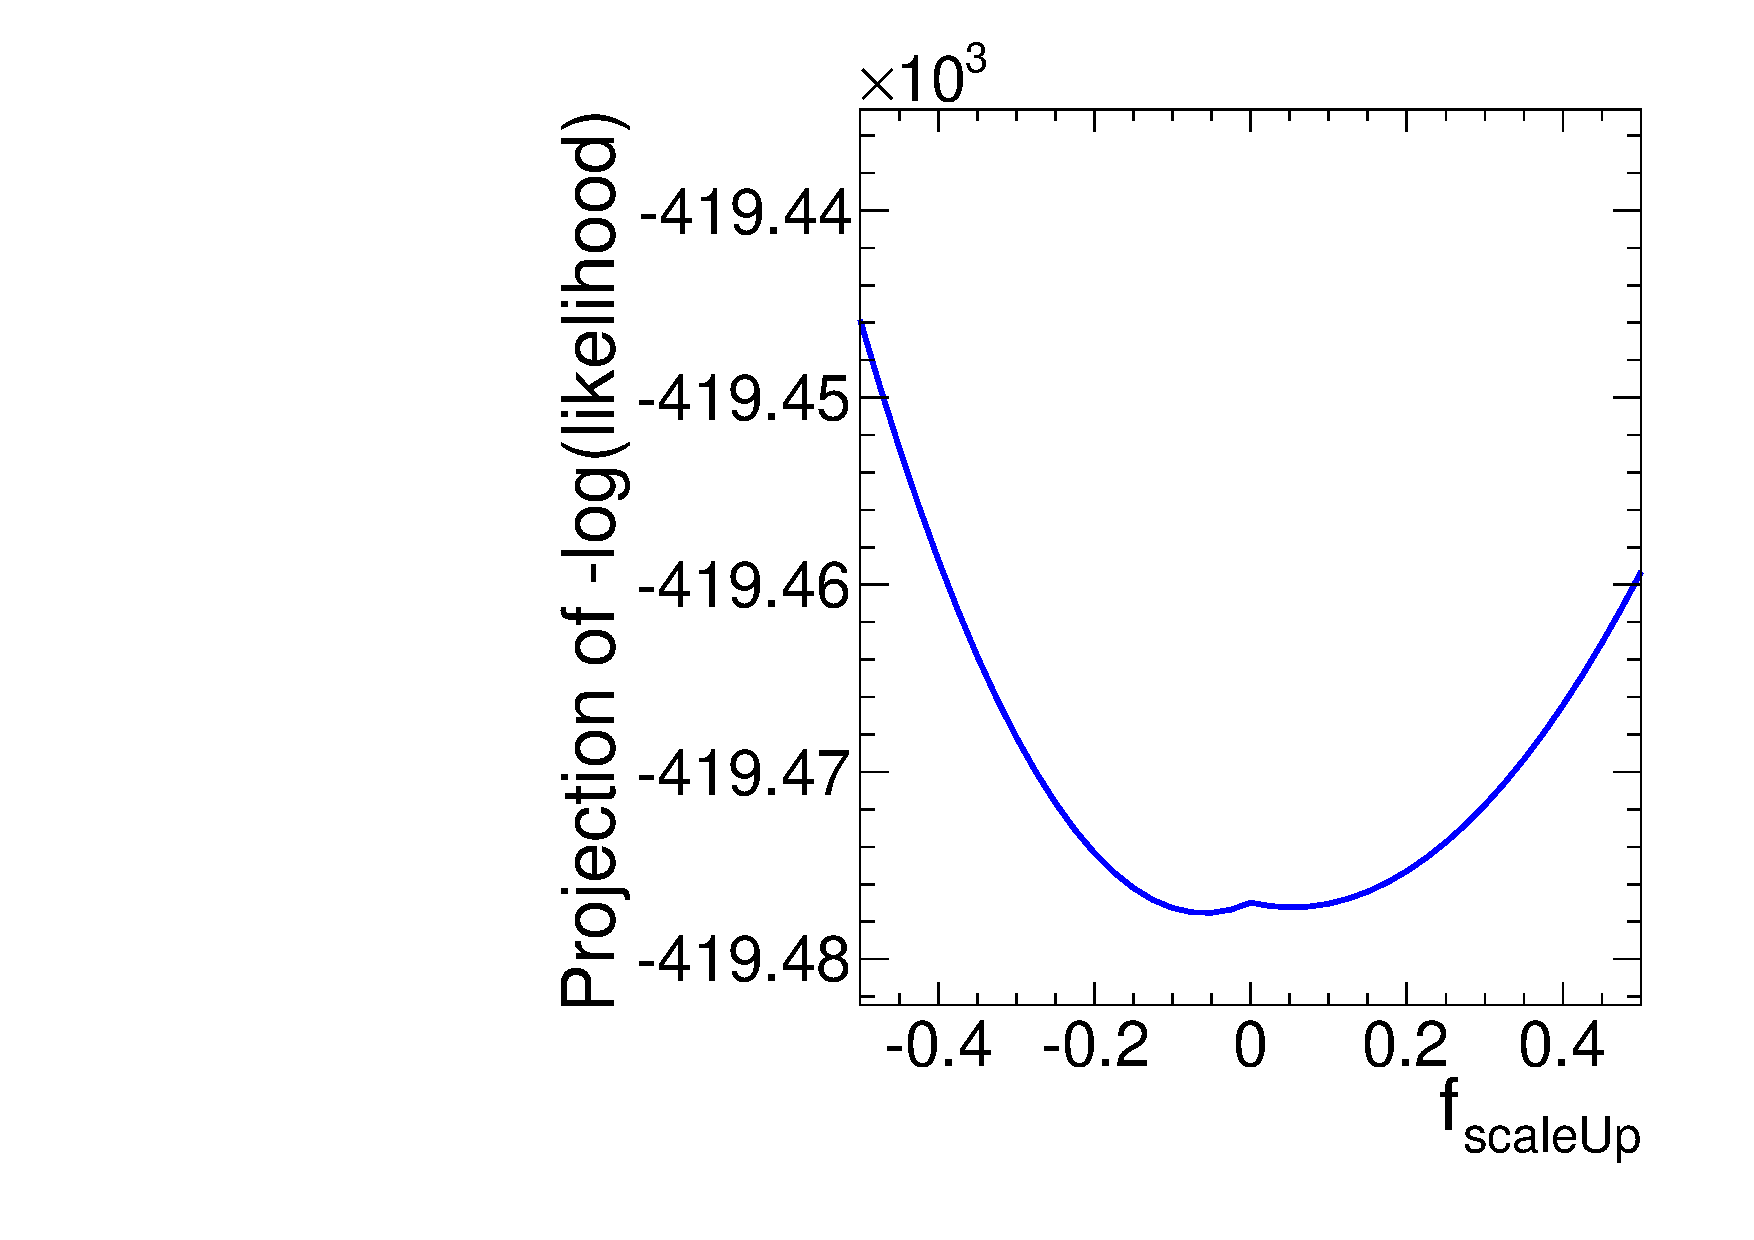
\includegraphics[width=0.48\textwidth]{figs/DibosonNLLfSU.pdf}
%    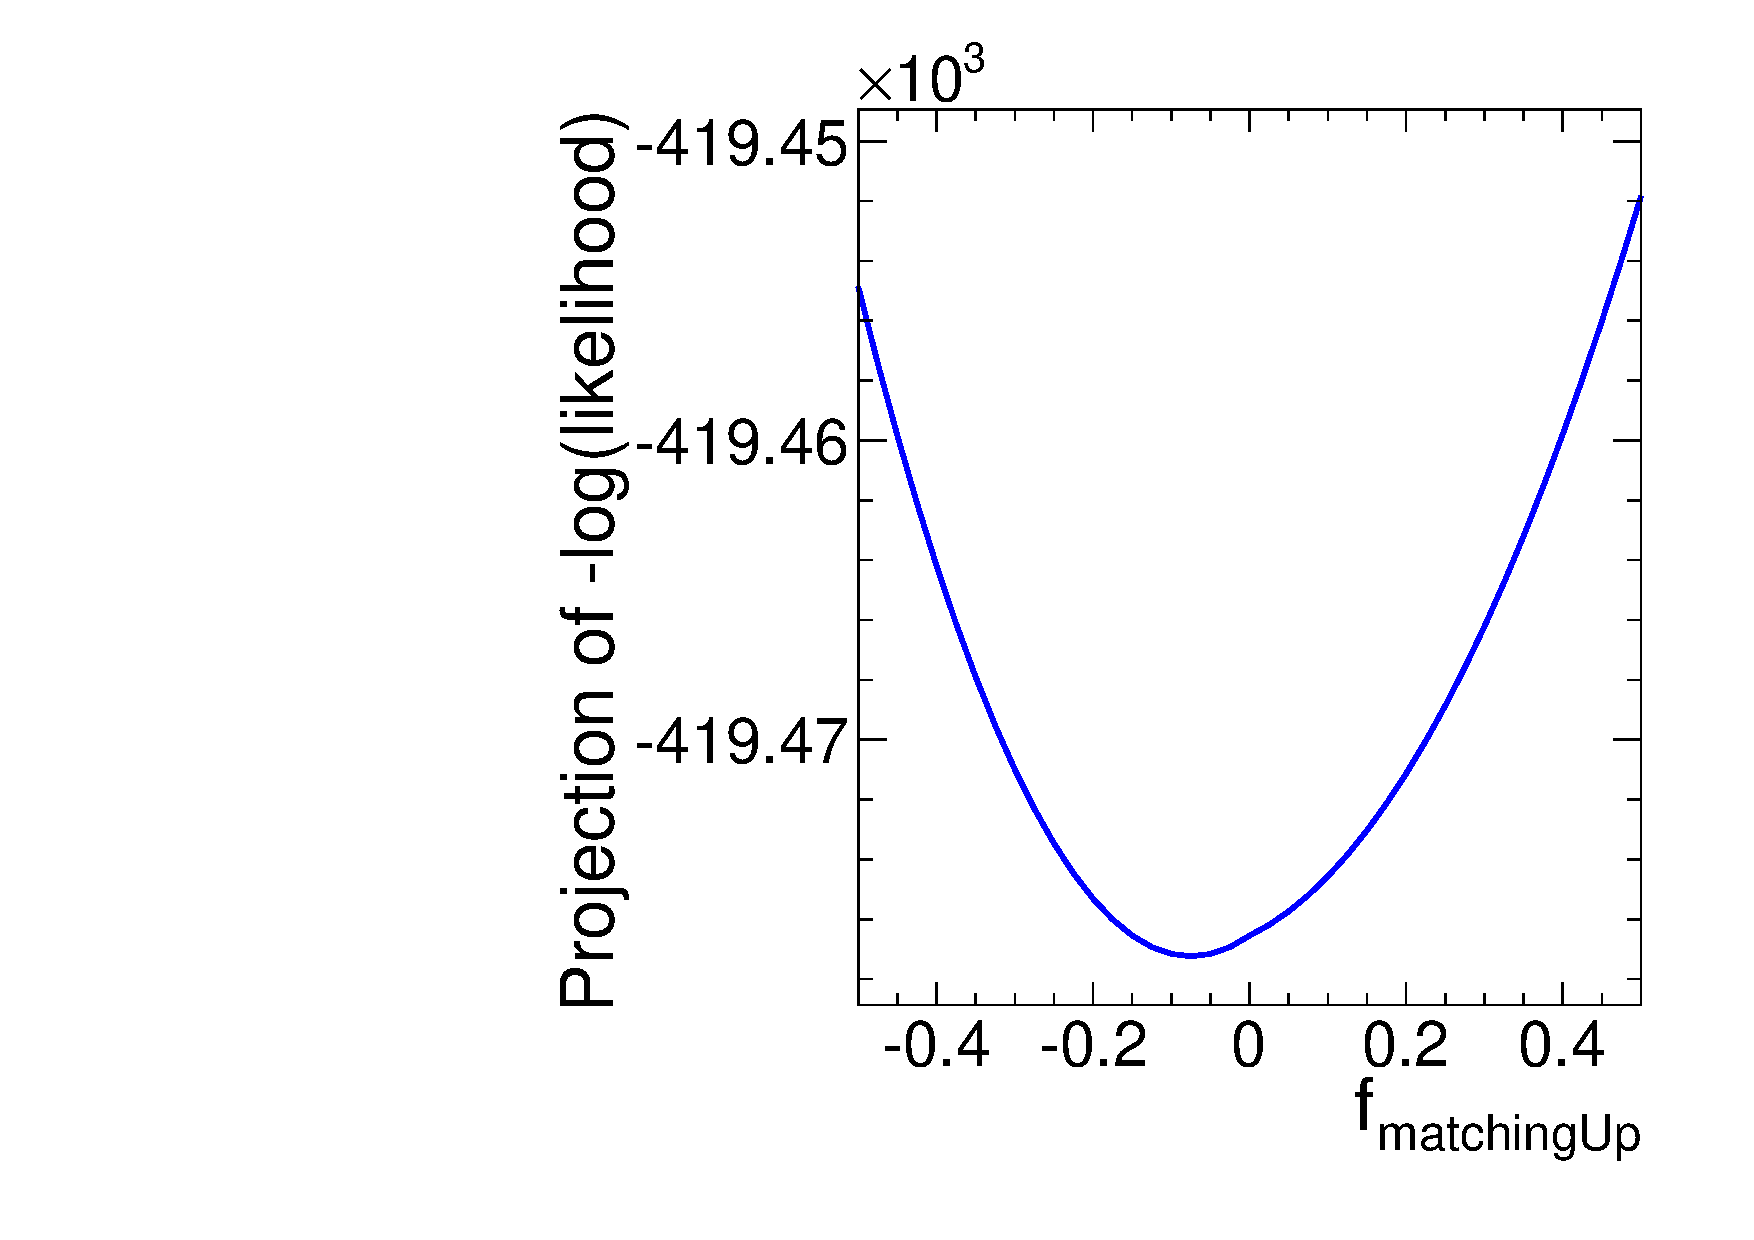
\includegraphics[width=0.48\textwidth]{figs/DibosonNLLfMU.pdf}
%    \caption{The scan of the negative log likelihood for the 
%factrization/renormalization and ME-PS matching scales. They have the 
%usual parabolic distribution with minimum near 0. The minimum values 
%correspond to the ones obtained in our nominal fit and listed in 
%Table~\ref{tab:wjetsscale}. }
%    \label{fig:q2NLLscan}}
%\end{figure}
%%%%%%%%%%%%%

%%%%%%%%%%%%%%%%%%%%%%%%%%%%%
\subsection{W+jets shape and normalization}
\label{sec:topsys}
Two parameter power law function is used to model the W+jets shape. So different parametric function of W+jets can affect the fit result. We use another expo $\times$ pow law parametric function to describe the W+jets MC shape shown in Figure~\ref{fig:WpJFit_Dijet_model2} to Figure~\ref{fig:dibosonFit_Dijet_model2_Pull}:
\begin{equation}
  \mathcal{F}_{W+\text{jets alternative fuction}} = exp(c\times{m_{jj}}) \times m_{jj}^{a_{0}}
\end{equation}
where $a_{0}$ and c parameters obtained from the fit to the Monte Carlo.
These W+jets alternative fuction shape paramters are also float in the fit. W+jets yield normalization scale factor determined by fitting on the BDT output distribution is listed in Table~\ref{tab:bdtfitcontrol}. We change the W+jets normalization scale factor according to the uncertainty determined from the BDT output distribution fit in the W+jets control region(Table~\ref{tab:bdtfitcontrol}).
%%%%%%%%%%%%%%%%%%%%%%%%%%%%%%%%%%%%%%%%%%%%%%%%%%%
\begin{figure}
\begin{center}
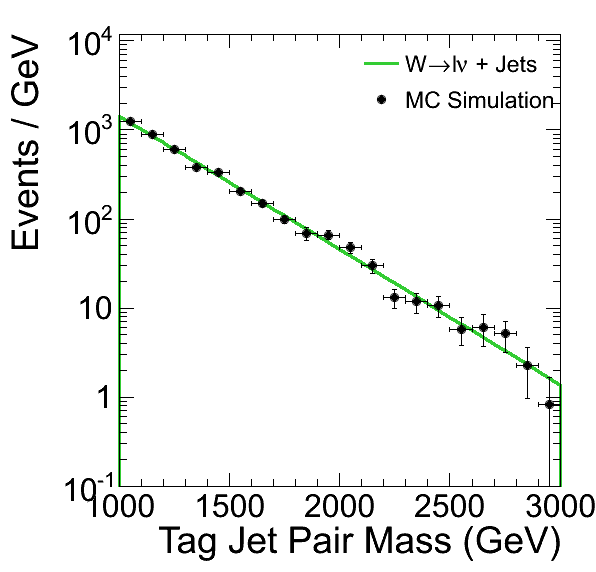
\includegraphics[width=0.45\textwidth]{figs/wpj/EWKW2jetstagjetmjj_WpJ_defaultfit_muon_Model_2_Validate.png}
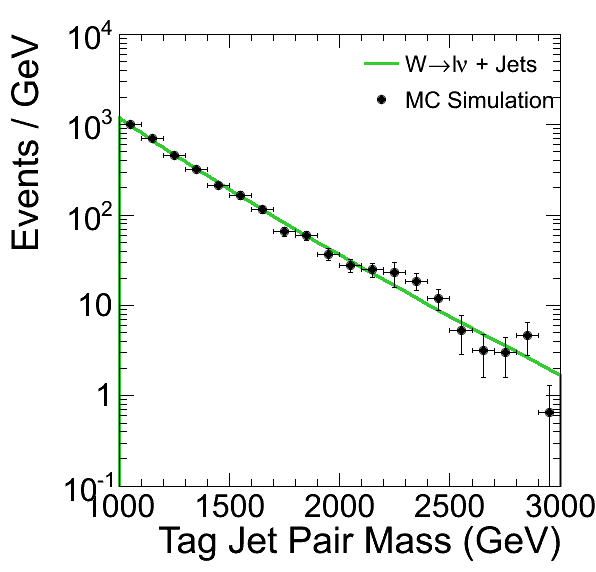
\includegraphics[width=0.45\textwidth]{figs/wpj/EWKW2jetstagjetmjj_WpJ_defaultfit_electron_Model_2_Validate.png}
\end{center}
\caption{\label{fig:dibosonFit} W+jets tagjet pair mass $m_{jj}$ shape with expo $\times$ pow law parametric function: projection of a fit to the W+jets MC for muons (left) and electrons (right).}
\label{fig:WpJFit_Dijet_model2}
\end{figure}

\begin{figure}
\begin{center}
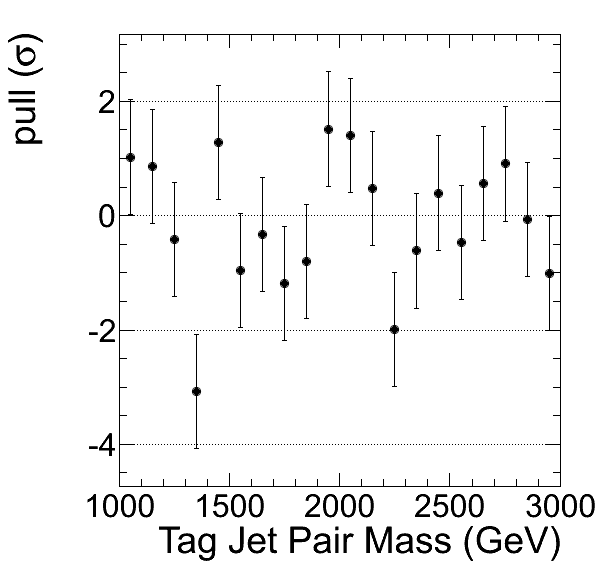
\includegraphics[width=0.45\textwidth]{figs/wpj/EWKW2jetstagjetmjj_WpJ_defaultfit_muon_Model_2_Validate_pull.png}
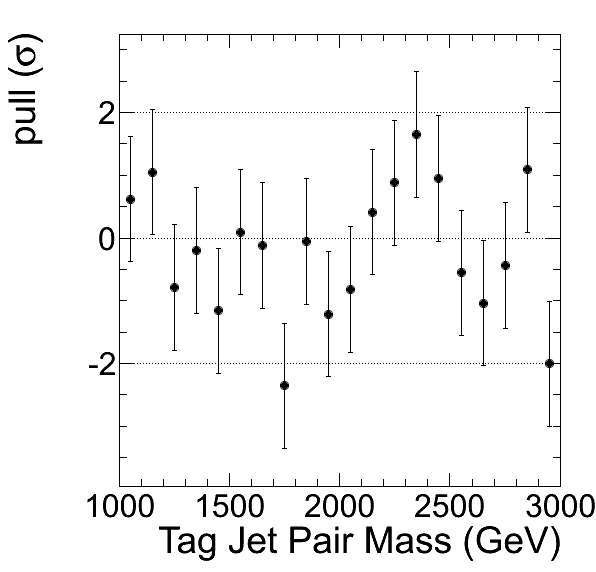
\includegraphics[width=0.45\textwidth]{figs/wpj/EWKW2jetstagjetmjj_WpJ_defaultfit_electron_Model_2_Validate_pull.png}
\end{center}
\caption{\label{fig:dibosonFit} W+jets tag jet pair mass $m_{jj}$ shape with expo $\times$ pow law parametric function: Pull distribution of a fit to the W+jets MC for muons (left) and electrons (right).}
\label{fig:dibosonFit_Dijet_model2_Pull}
\end{figure}
%%%%%%%%%%%%%%%%%%%%%%%%%%%%%%%%%%%%%%%%%%%%
\subsection{Jet Energy Scale}
\label{sec:topw}
A dedicated analysis of 2010 data by the JetMET group showed that the jet energy
uncertainty for a generic particle-flow jet is within 3\% and the jet energy resolution
(JER) uncertainty is within 10\%.  For more details, see
Refs.~\cite{jetsyst,jetsyst2}.  The systematic uncertainties in the
JES and JER can affect our signal acceptance and the tagjet pair invariant mass $m_{jj}$ distribution.
Figure~\ref{fig:topJECComparison} to Figure~\ref{fig:ewkw2jetsJECComparison} shows a comparison of TTbar shape and EWK W+2jets signal shape
obtained using default jet energy scale with those obtained by using 
$\pm 1\sigma$ variation in the default scale.
%In the present analysis, we performed several studies to cross check 
%and constrain the JES uncertainties.
%Two such studies are described 
%below. We determine that the average uncertainty in the JES for the 
%jet kinematics relevant to the present analysis is at the level below 1\% 
%and uncertainty in JER is at the level of 10\%. %These are in agreement 
%with Refs.~\cite{jetsyst,jetsyst2} for jets of $p_T > 35$~\gev and 
%$|\eta|<2.4$. The effect of propagating these uncertainties to the 
%signal acceptance and diboson yields is minuscule. 
%%%%%%%%%%%%
%%%%%%%%%%%%
\begin{figure}{\centering
    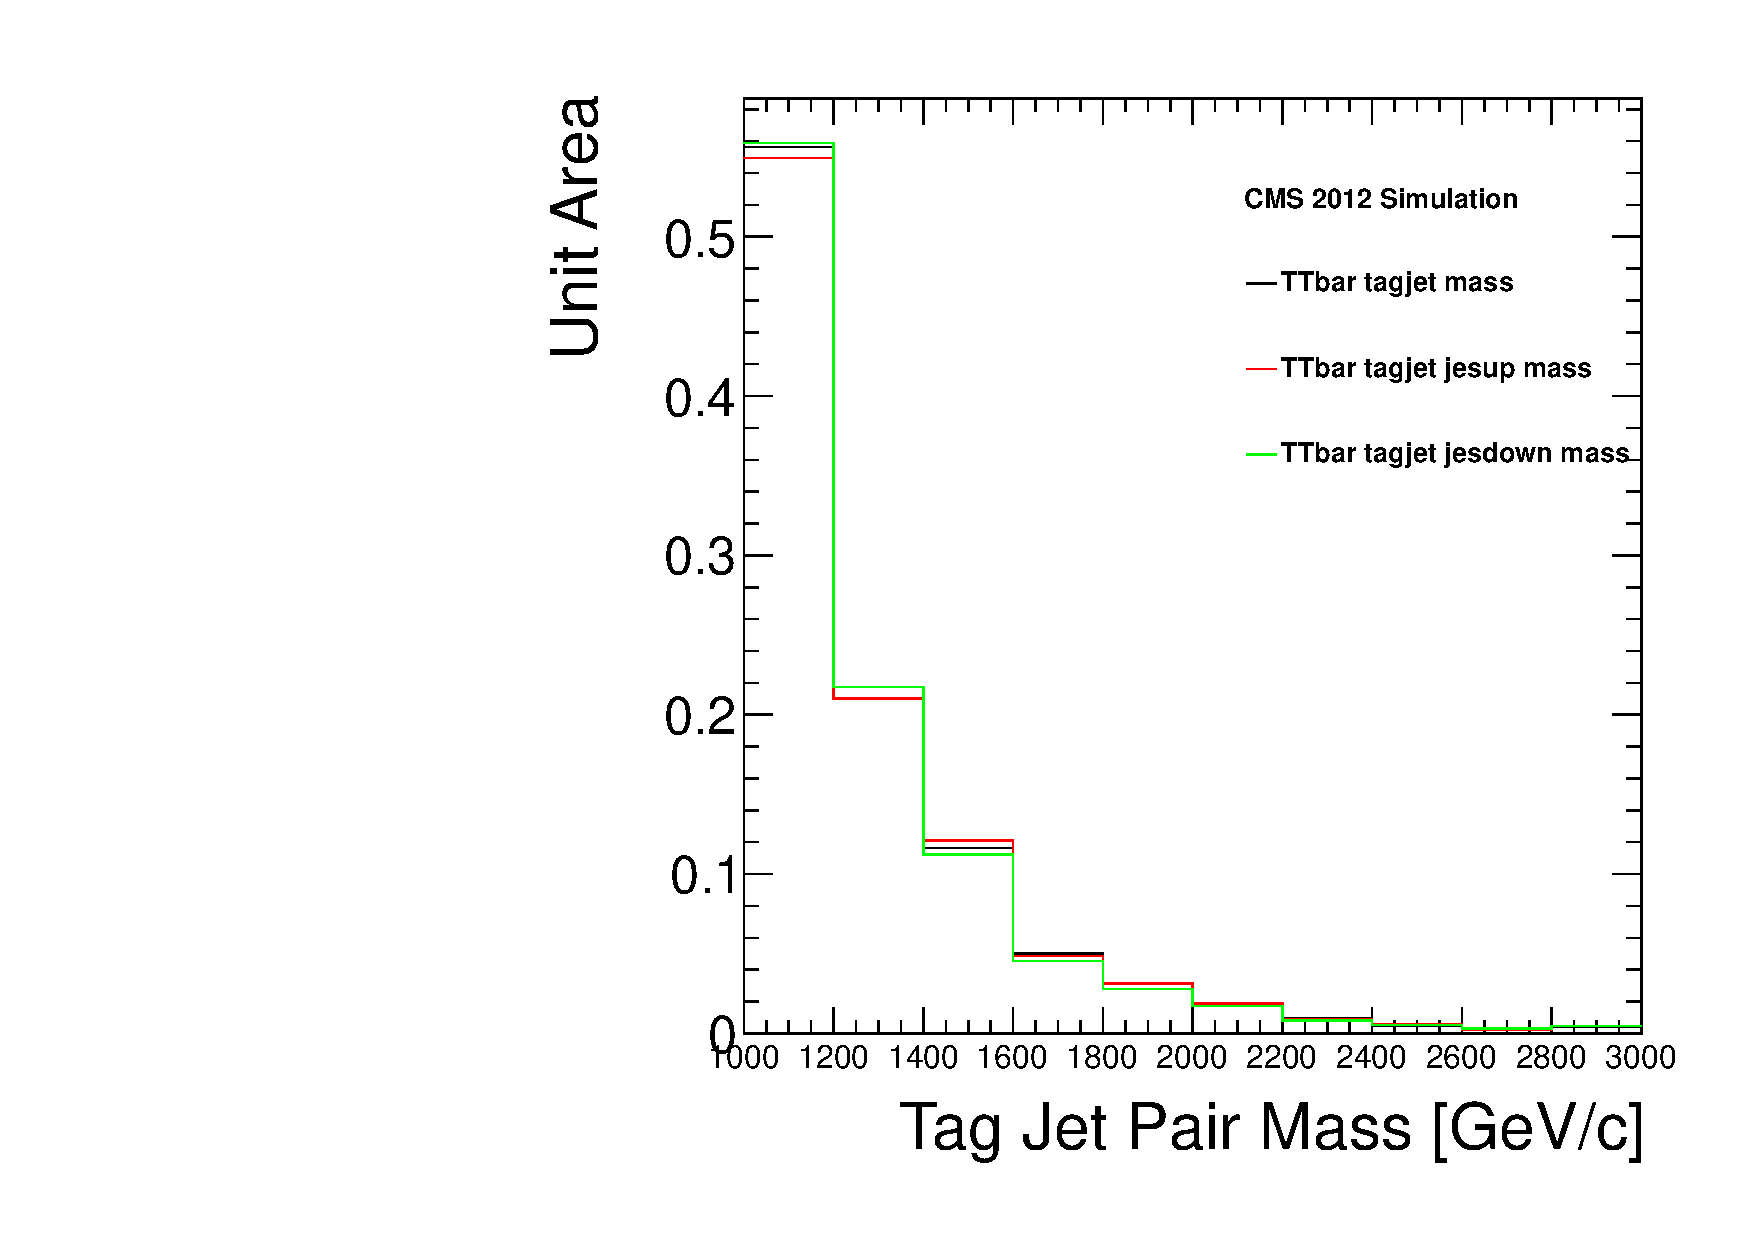
\includegraphics[width=0.49\textwidth]{figs/systematic/mu_TTbar_tagjet_mass_tagjet_jesup_mass_tagjet_jesdown_mass_topjes_syscompare.pdf}
    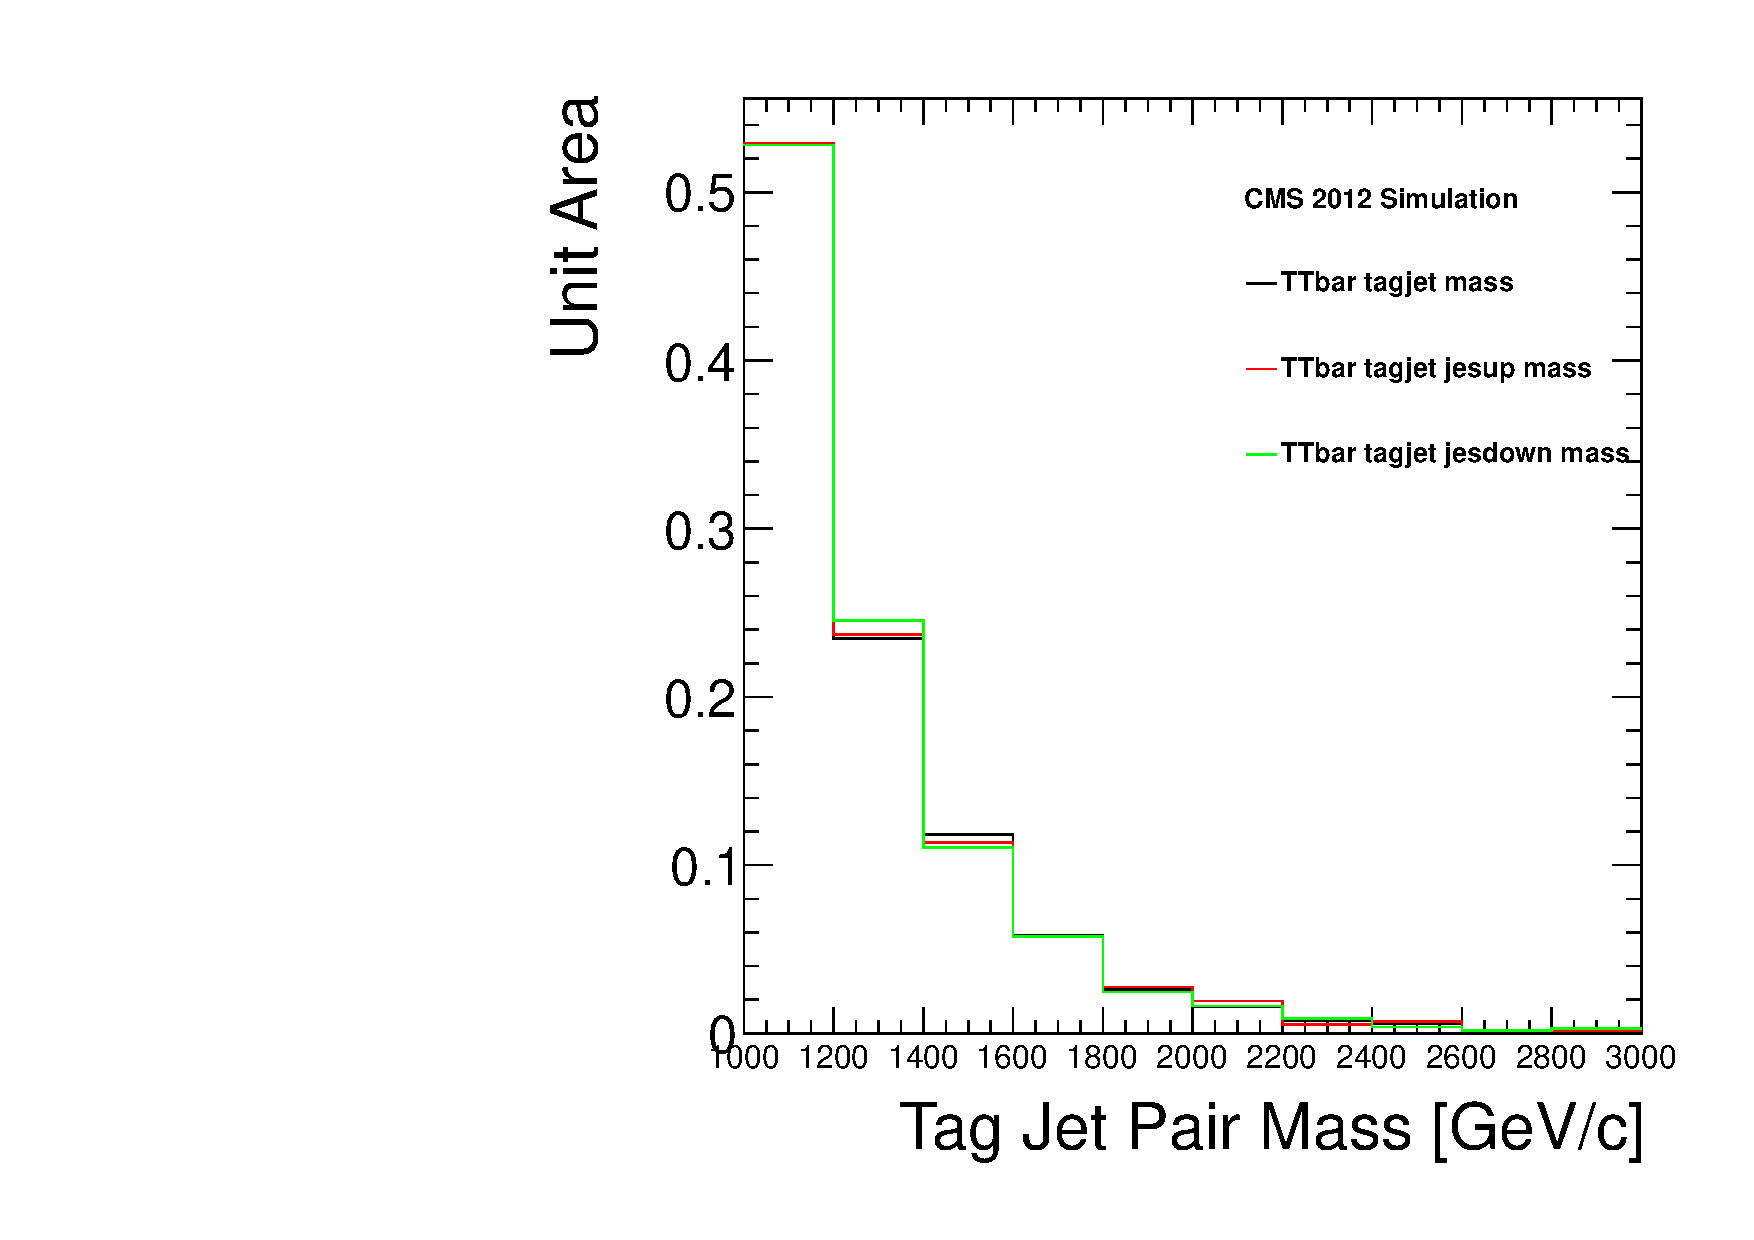
\includegraphics[width=0.49\textwidth]{figs/systematic/el_TTbar_tagjet_mass_tagjet_jesup_mass_tagjet_jesdown_mass_topjes_syscompare.pdf}
    \caption{Comparison of TTbar shape using default JES and 
    using $\pm 1\sigma$ variation in JES: muons(left) and electrons(right). }
    \label{fig:topJECComparison}}
\end{figure}
%%%%%%%%%%%%%%%%%%
\begin{figure}{\centering
    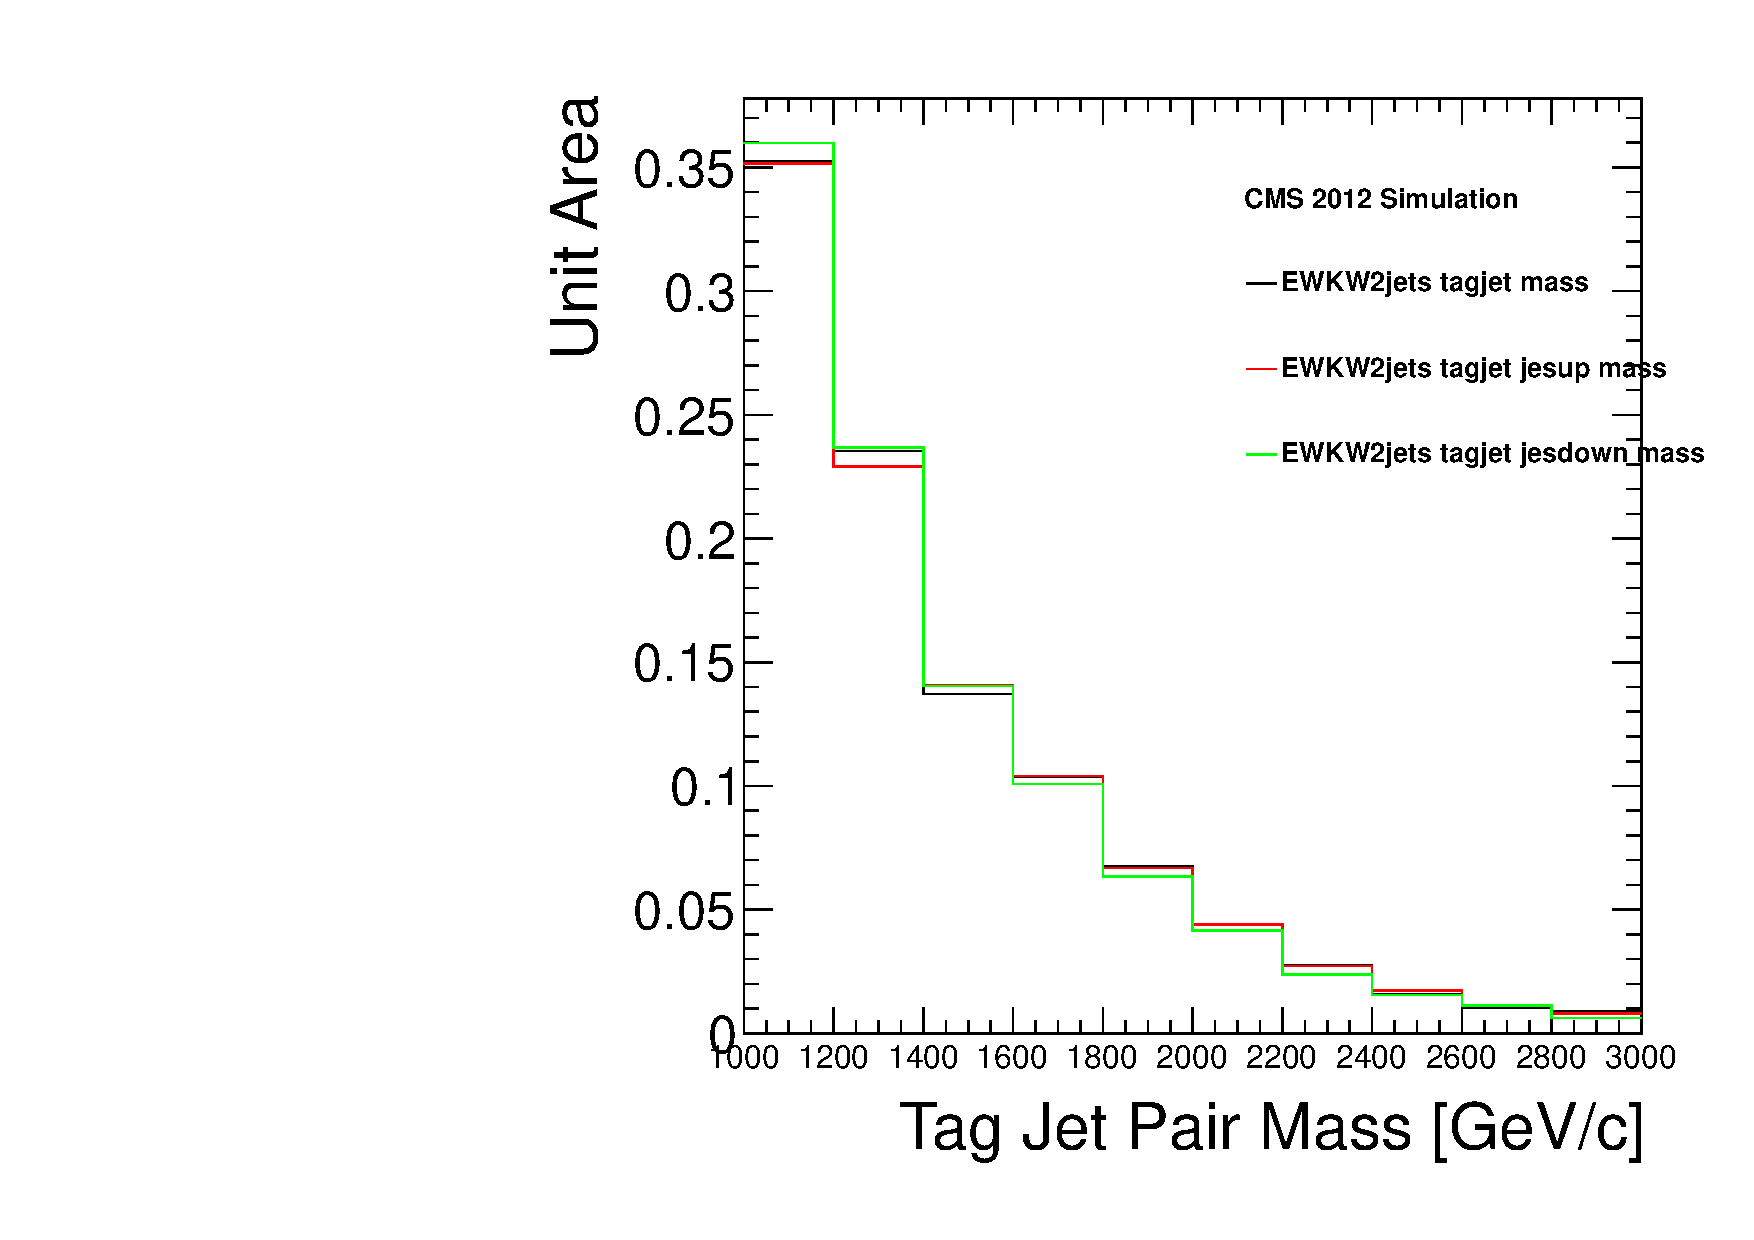
\includegraphics[width=0.49\textwidth]{figs/systematic/mu_EWKW2jets_tagjet_mass_tagjet_jesup_mass_tagjet_jesdown_mass_ewkw2jetsjes_syscompare.pdf}
    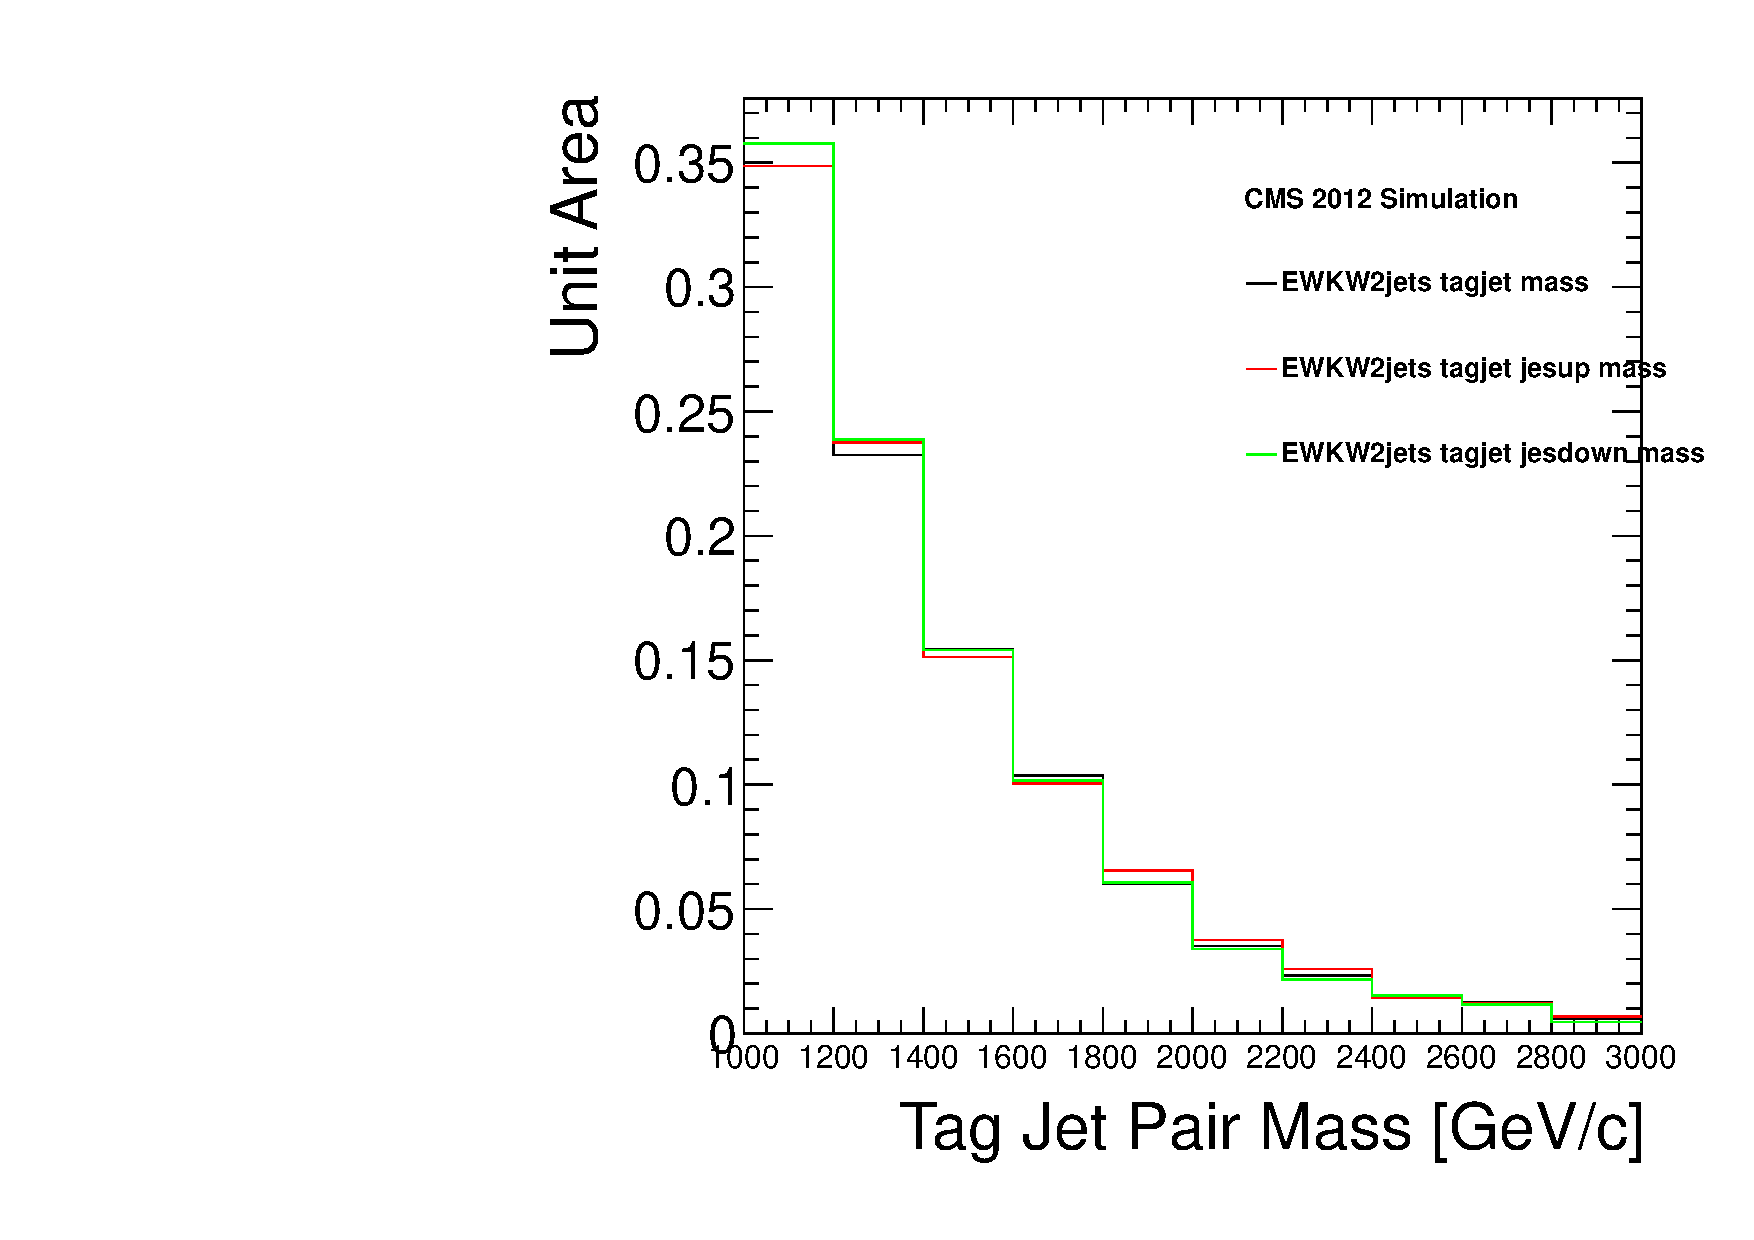
\includegraphics[width=0.49\textwidth]{figs/systematic/el_EWKW2jets_tagjet_mass_tagjet_jesup_mass_tagjet_jesdown_mass_ewkw2jetsjes_syscompare.pdf}
    \caption{Comparison of EWKW2jets signal shape using default JES and 
    using $\pm 1\sigma$ variation in JES: muons(left) and electrons(right). }
    \label{fig:ewkw2jetsJECComparison}}
\end{figure}
%%%%%%%%%%%%%%%%%%
\subsection{Jet Energy Resolution}
\label{sec:jer}
Jet energy resolution systematic uncetrainty is caused by different jet energy performance between data and MC. First we calcualte the JER $\sigma_{MC}$ by using the EWK W+2jets signal sample. The detail calculation is in the Appendex ~\ref{app:jer}. The detail JER with several jet $p_{T}$ and $\eta$ bins is listed in Table~\ref{tab:jetjer}. We then gaussian smear the jet pt of the MC sample with the $\sigma_{data}$ following the steps on twiki:https://twiki.cern.ch/twiki/bin/viewauth/CMS/JetResolution. 

Figure~\ref{fig:topJERComparison} to Figure~\ref{fig:ewkw2jetsJERComparison} shows a comparison of TTbar shape and EWK W+2jets signal shape obtained using default jet energy resolution with those obtained by using $\pm 1\sigma$ variation in the default scale.
%%%%%%%%%%%%%%%%%%%%%%%%%%%%%%%%%%%%
\begin{table}[htb]
\centering 
\scalebox{0.70}{
\begin{tabular}{|c|c|c|c|c|}
\hline
$p_{\textnormal{T,min}}$ & $p_{\textnormal{T,max}}$ & $\eta_{\textnormal{min}}$ & $\eta_{\textnormal{max}}$ & JER $\sigma_{MC}$\\
$[\GeVc]$         & $[\GeVc]$         &                     &                     &  \\
\hline
\hline
30.0 & 50.0 & 0.0 & 0.5 & 0.1446 \\
30.0 & 50.0 & 0.5 & 1.1 & 0.1254 \\
30.0 & 50.0 & 1.1 & 1.7 & 0.1511 \\
30.0 & 50.0 & 1.7 & 2.3 & 0.1475 \\
30.0 & 50.0 & 2.3 & 5.0 & 0.1301 \\
50.0 & 70.0 & 0.0 & 0.5 & 0.1156 \\
50.0 & 70.0 & 0.5 & 1.1 & 0.1288 \\
50.0 & 70.0 & 1.1 & 1.7 & 0.1455 \\
50.0 & 70.0 & 1.7 & 2.3 & 0.1266 \\
50.0 & 70.0 & 2.3 & 5.0 & 0.1346 \\
70.0 & 100.0 & 0.0 & 0.5 & 0.1106 \\
70.0 & 100.0 & 0.5 & 1.1 & 0.1113 \\
70.0 & 100.0 & 1.1 & 1.7 & 0.1166 \\
70.0 & 100.0 & 1.7 & 2.3 & 0.1035 \\
70.0 & 100.0 & 2.3 & 5.0 & 0.1131 \\
100.0 & 200.0 & 0.0 & 0.5 & 0.0921 \\
100.0 & 200.0 & 0.5 & 1.1 & 0.0939 \\
100.0 & 200.0 & 1.1 & 1.7 & 0.0970 \\
100.0 & 200.0 & 1.7 & 2.3 & 0.0814 \\
100.0 & 200.0 & 2.3 & 5.0 & 0.0878 \\
200.0 & 300.0 & 0.0 & 0.5 & 0.0785 \\
200.0 & 300.0 & 0.5 & 1.1 & 0.0737 \\
200.0 & 300.0 & 1.1 & 1.7 & 0.0754 \\
200.0 & 300.0 & 1.7 & 2.3 & 0.0624 \\
200.0 & 300.0 & 2.3 & 5.0 & 0.0668 \\
300.0 & 500.0 & 0.0 & 0.5 & 0.0648 \\
300.0 & 500.0 & 0.5 & 1.1 & 0.0704 \\
300.0 & 500.0 & 1.1 & 1.7 & 0.0685 \\
300.0 & 500.0 & 1.7 & 2.3 & 0.0545 \\
300.0 & 500.0 & 2.3 & 5.0 & 0.0652 \\
\hline
\end{tabular}}
\caption{Jet Energy Resolution in the MC jet $p_{T}$ and $\eta$ bins}
\label{tab:jetjer} 
\end{table}
%%%%%%%%%%%%%%%%%%%%%%%%%%%%%%
\begin{figure}[htb]
{\centering
    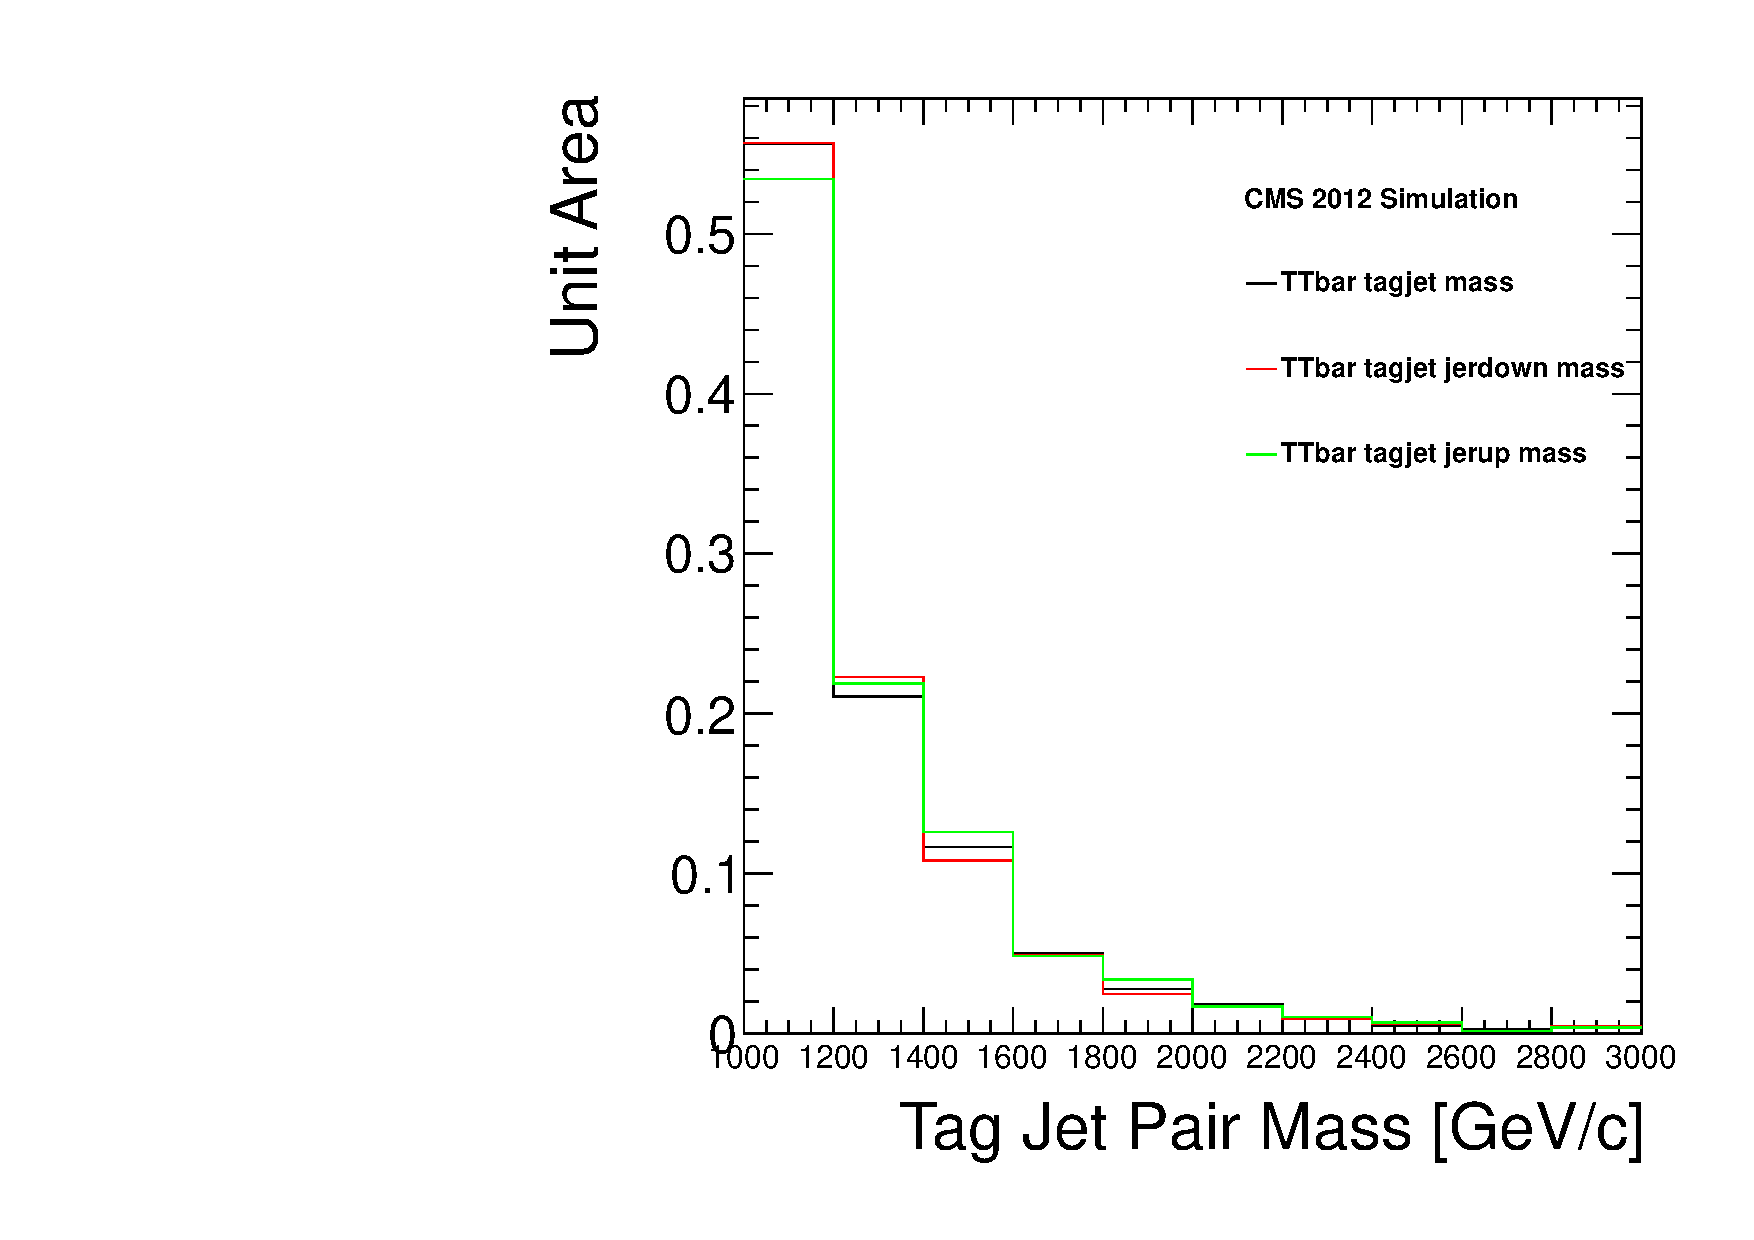
\includegraphics[width=0.49\textwidth]{figs/systematic/mu_TTbar_tagjet_mass_tagjet_jerup_mass_tagjet_jerdown_mass_topjer_syscompare.pdf}
    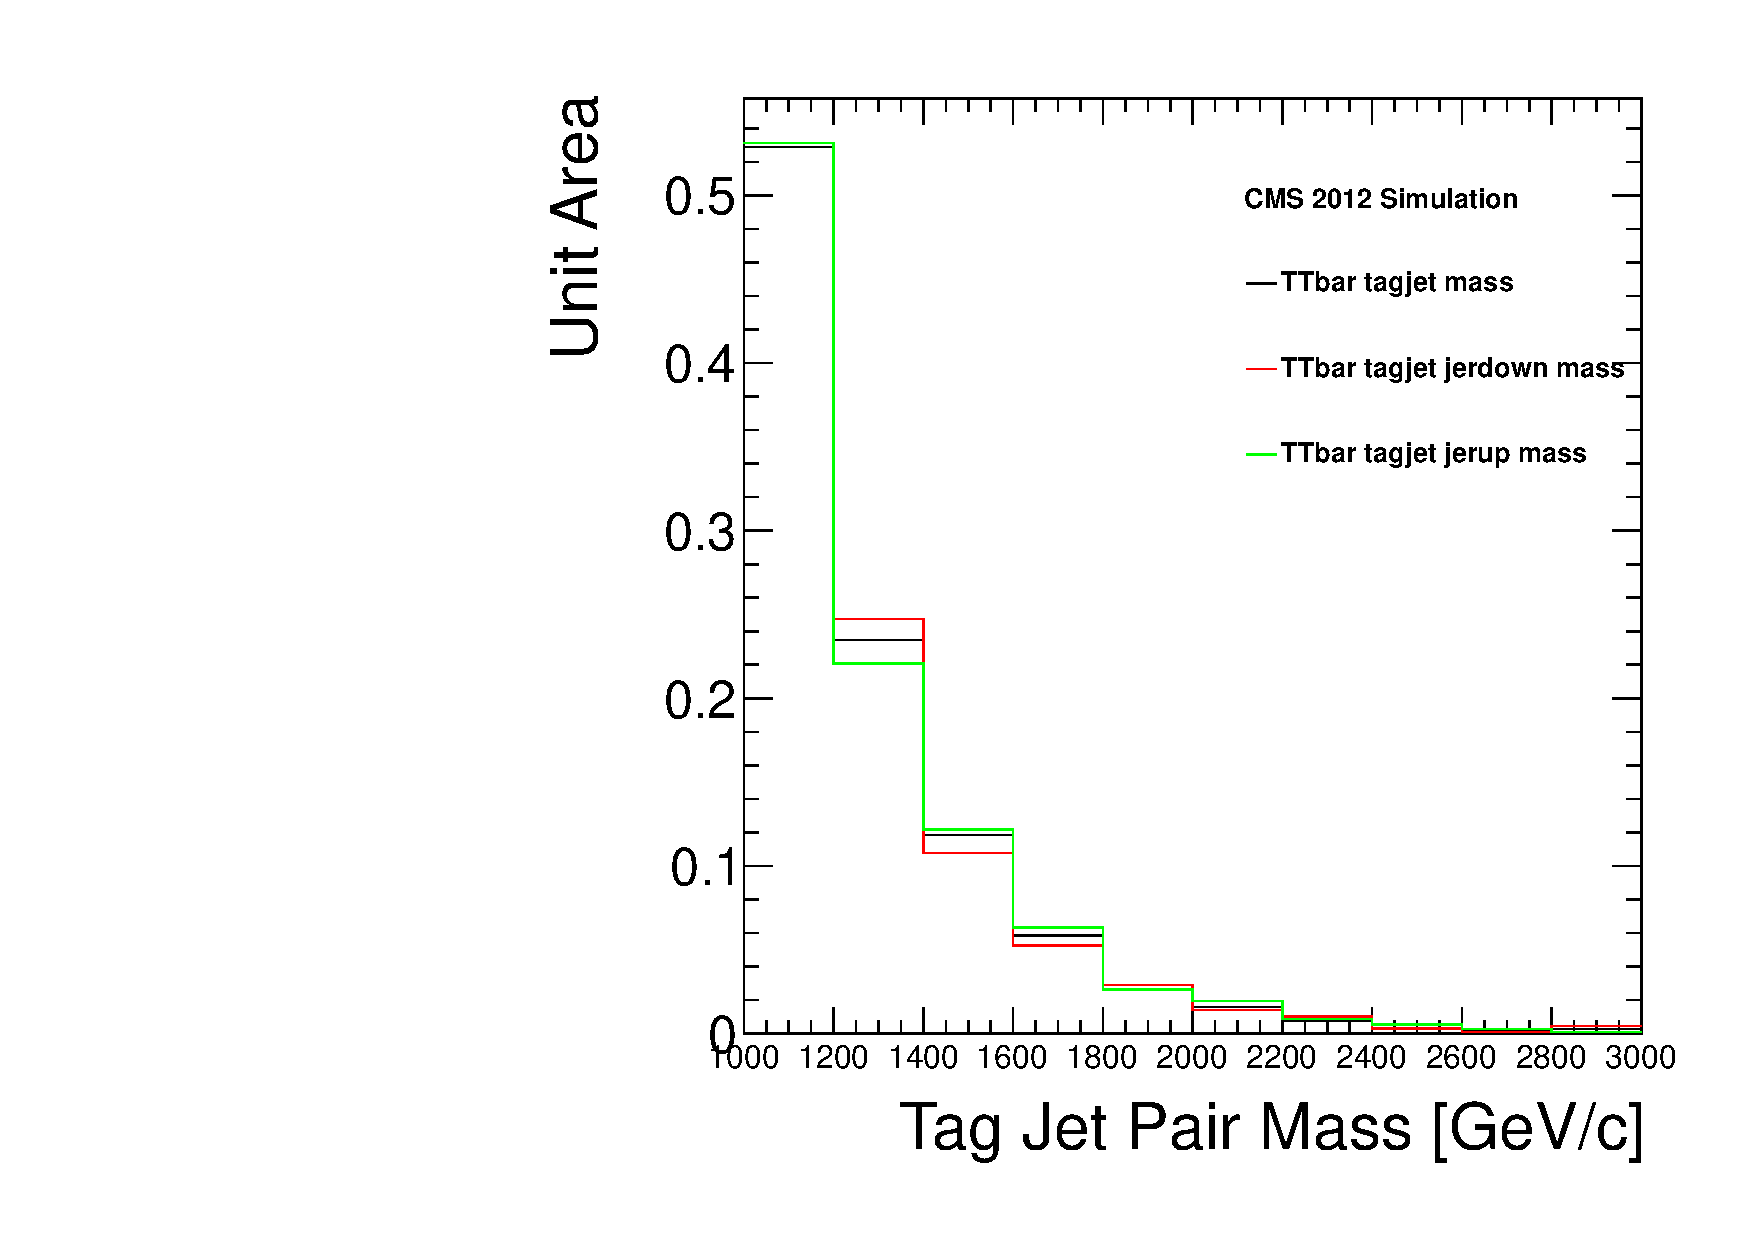
\includegraphics[width=0.49\textwidth]{figs/systematic/el_TTbar_tagjet_mass_tagjet_jerup_mass_tagjet_jerdown_mass_topjer_syscompare.pdf}
    \caption{Comparison of TTbar shape using default JER and 
    using $\pm 1\sigma$ variation in JER: muons(left) and electrons(right). }
    \label{fig:topJERComparison}}
\end{figure}
%%%%%%%%%%%%%%%%%%
\begin{figure}[htb]
{\centering
    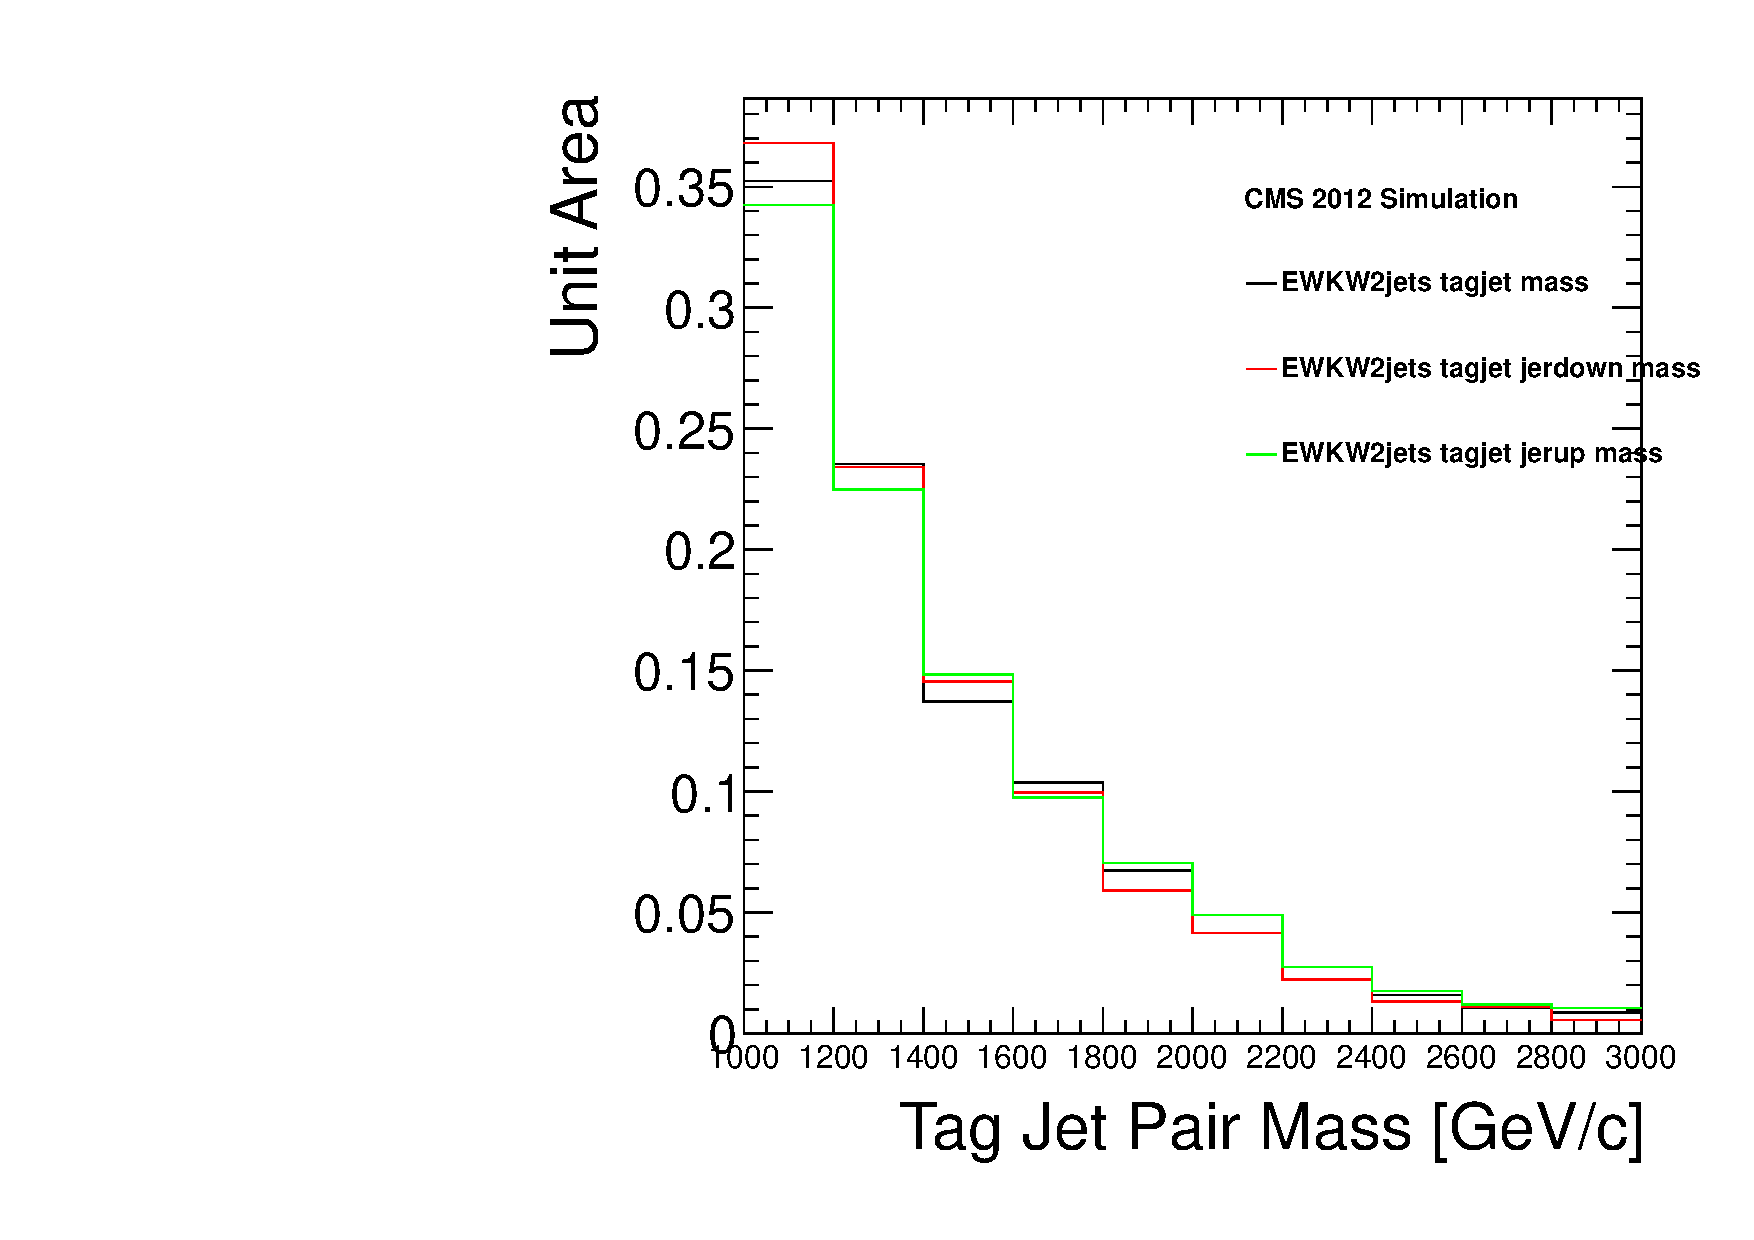
\includegraphics[width=0.49\textwidth]{figs/systematic/mu_EWKW2jets_tagjet_mass_tagjet_jerup_mass_tagjet_jerdown_mass_ewkw2jetsjer_syscompare.pdf}
    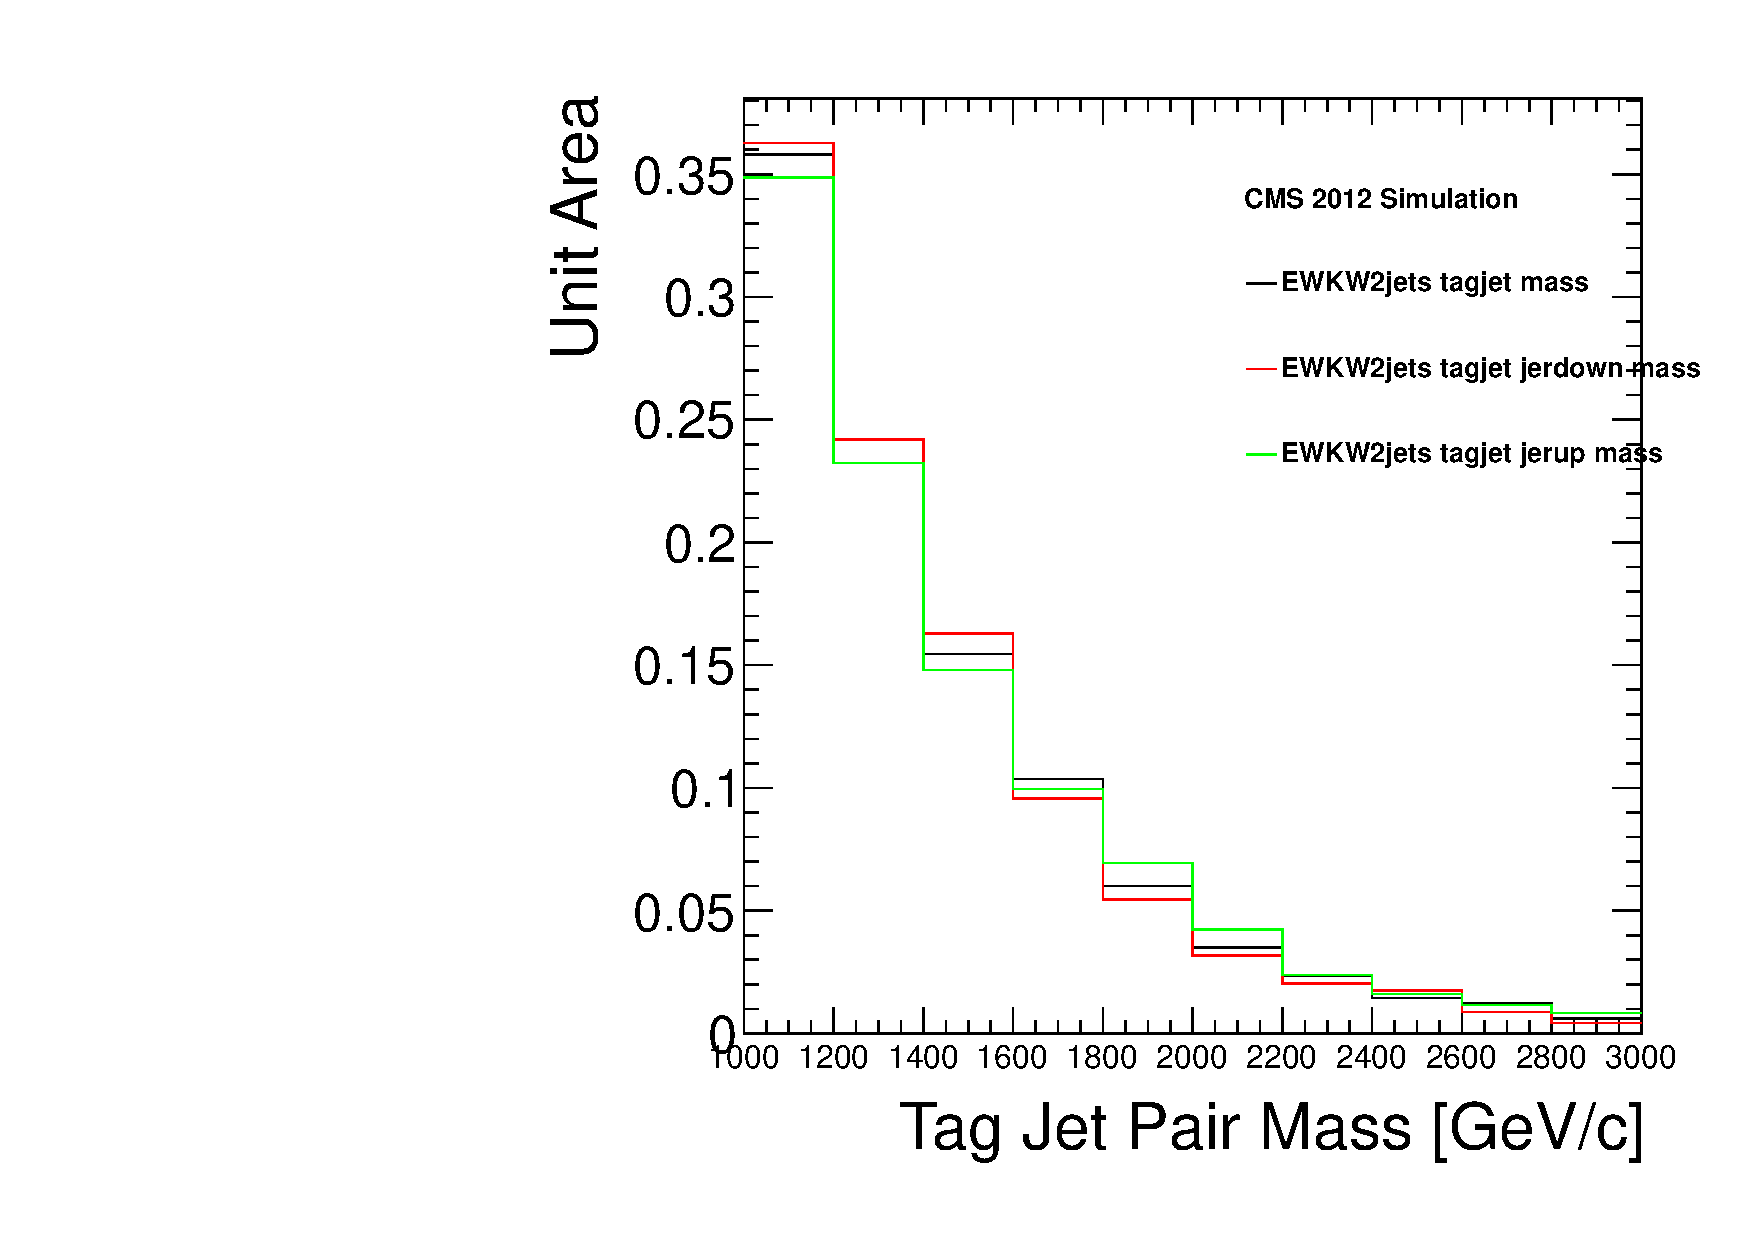
\includegraphics[width=0.49\textwidth]{figs/systematic/el_EWKW2jets_tagjet_mass_tagjet_jerup_mass_tagjet_jerdown_mass_ewkw2jetsjer_syscompare.pdf}
    \caption{Comparison of EWKW2jets signal shape using default JER and 
    using $\pm 1\sigma$ variation in JER: muons(left) and electrons(right). }
    \label{fig:ewkw2jetsJERComparison}}
\end{figure}
%%%%%%%%%%%%%%%%%%

%%%%%%%%%%%%
%%%%%%%%%%%%
%%%%%%%%%%%%
%\subsubsection{Scan of jet energy scale}
%In this study we scan the JES from -5\% to +5\% and repeat the fit. 
%We performed  this test in a subset of the muon data. 
%The $\chi^2$ of the fit is plotted in
%Figure~\ref{fig:JESScanchi2} as a function of the JES shift. 
%
%The minimum in $\chi^2$ is consistent
%with the value obtained from hadronic W candidates in top
%quark events (described below) and the fit has a stable, well defined minimum. 
%Note that the above study serves a crosscheck.
%%%%%%%%%%%%%
%\begin{figure}[h!] {\centering
%    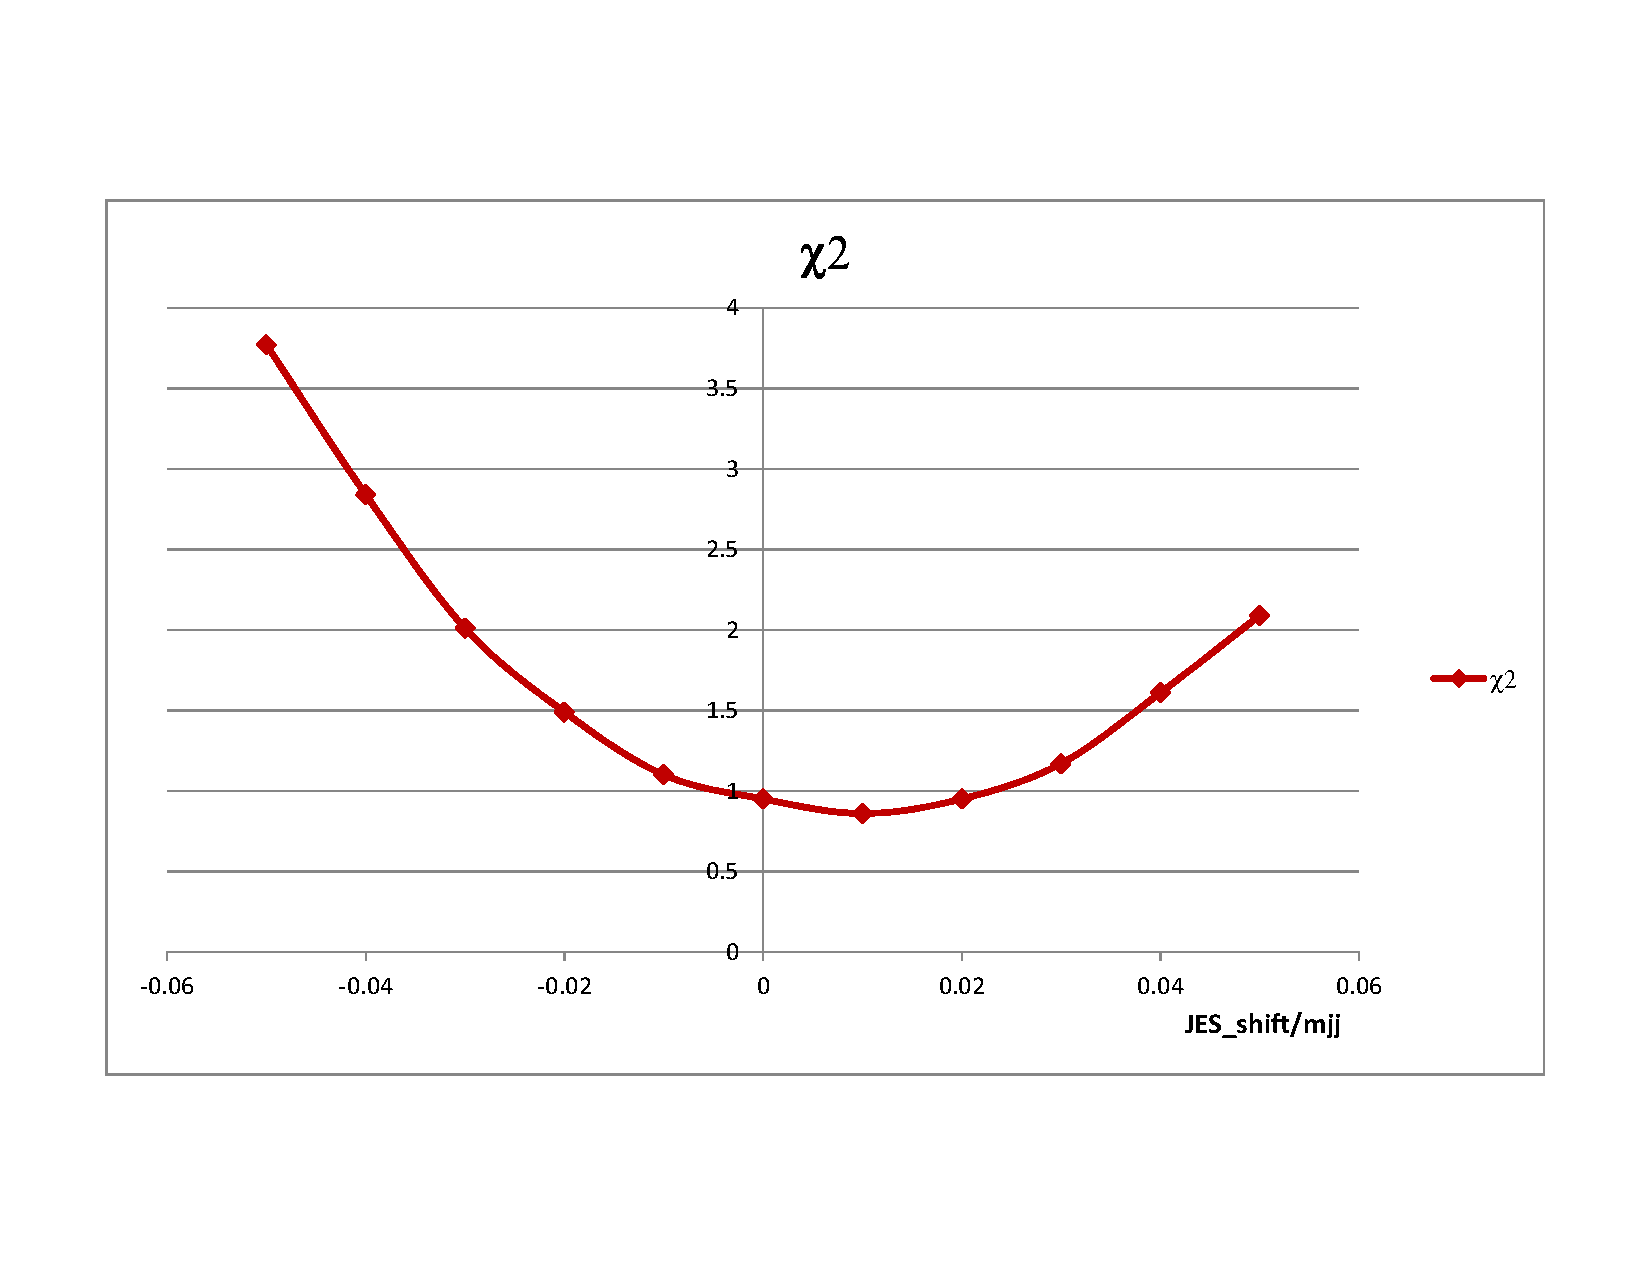
\includegraphics[width=0.5\textwidth]{figs/JES_scan.pdf}
%    \caption{$\chi^2$ of the fit vs JES shift for muon no b-tag data.}
%    \label{fig:JESScanchi2}}
%\end{figure}
%%%%%%%%%%%%

%%%%%%%%%%%%%%%%%%%%%%%%%%%%%
\subsection{$t\bar{t}$ shape modeling and normalization}
\label{sec:ttbar_resulved}

At LHC the top pair production rate is fairly large, almost fifty times larger than the electroweak W2jets production
rate. According to the Standard Model, the top quark decays into $W$
boson and $b$ quark with branching fraction of about 100\%. When we
select events in which one $W$ boson decays leptonically
(\textit{i.e.}, $W\to e\nu, \mu\nu$) and the other $W$ boson decays
into quark pairs thus leading to a semileptonic final state, then the
signal purity is very high.  The final state consists of a high energy
lepton, large missing $E_T$, and four jets(jet1 $p_{T}>$ 60 GeV and jet2 $p_{T}>$50 GeV) of which two are
$b$-tagged, at least two anti-btagged jets. 
%The hadronic W candidates are formed from two anti-btagged jets.  
The invariant mass of the  the leading jet and second leading jet is shown in
Fig.~\ref{fig:topw:mu_MC}. More cross check distributions of the TTbar control region can be found in Appendix~\ref{app:ttbar}. We find reasonable agreement between Top MC sample and data comparsion. 
Besides cross checking the ttbar modeling in the data, we also use different top samples with different generators and shower models(1. aMC@NLO + Herwig; 2. Powheg + Pythia) to replace the default top Madgraph shapes. The new top samples shape modeling can be found in Fig.~\ref{fig:mu_MC_topaMCNLO} to Fig.~\ref{fig:mu_MC_toppowheg_pull}.
%As an alternative, we convolve the MC templates with a Gaussian resolution function and
%repeat the fit on the control sample data (Fig.~\ref{fig:topw:mu_ConvolvedMC}). The Gaussian parameters returned by the fit are $\mu=4.28\pm 0.50$, $\sigma=3.23\pm 0.49$~GeV. They are subsequently used for convolved template fit studies presented in section~\ref{sec:convolvedMCfit}. However, the $W$ mass resolution is dominated by the resolution of the jet energy measurement, with JES systematics accounted for as described in section~\ref{sec:topw}.
%%%%%%%%%%%%%%%%%%%%%
%%%%%%%%%%%%%%%%%%%%%
\begin{figure}[htb] 
  {\centering
    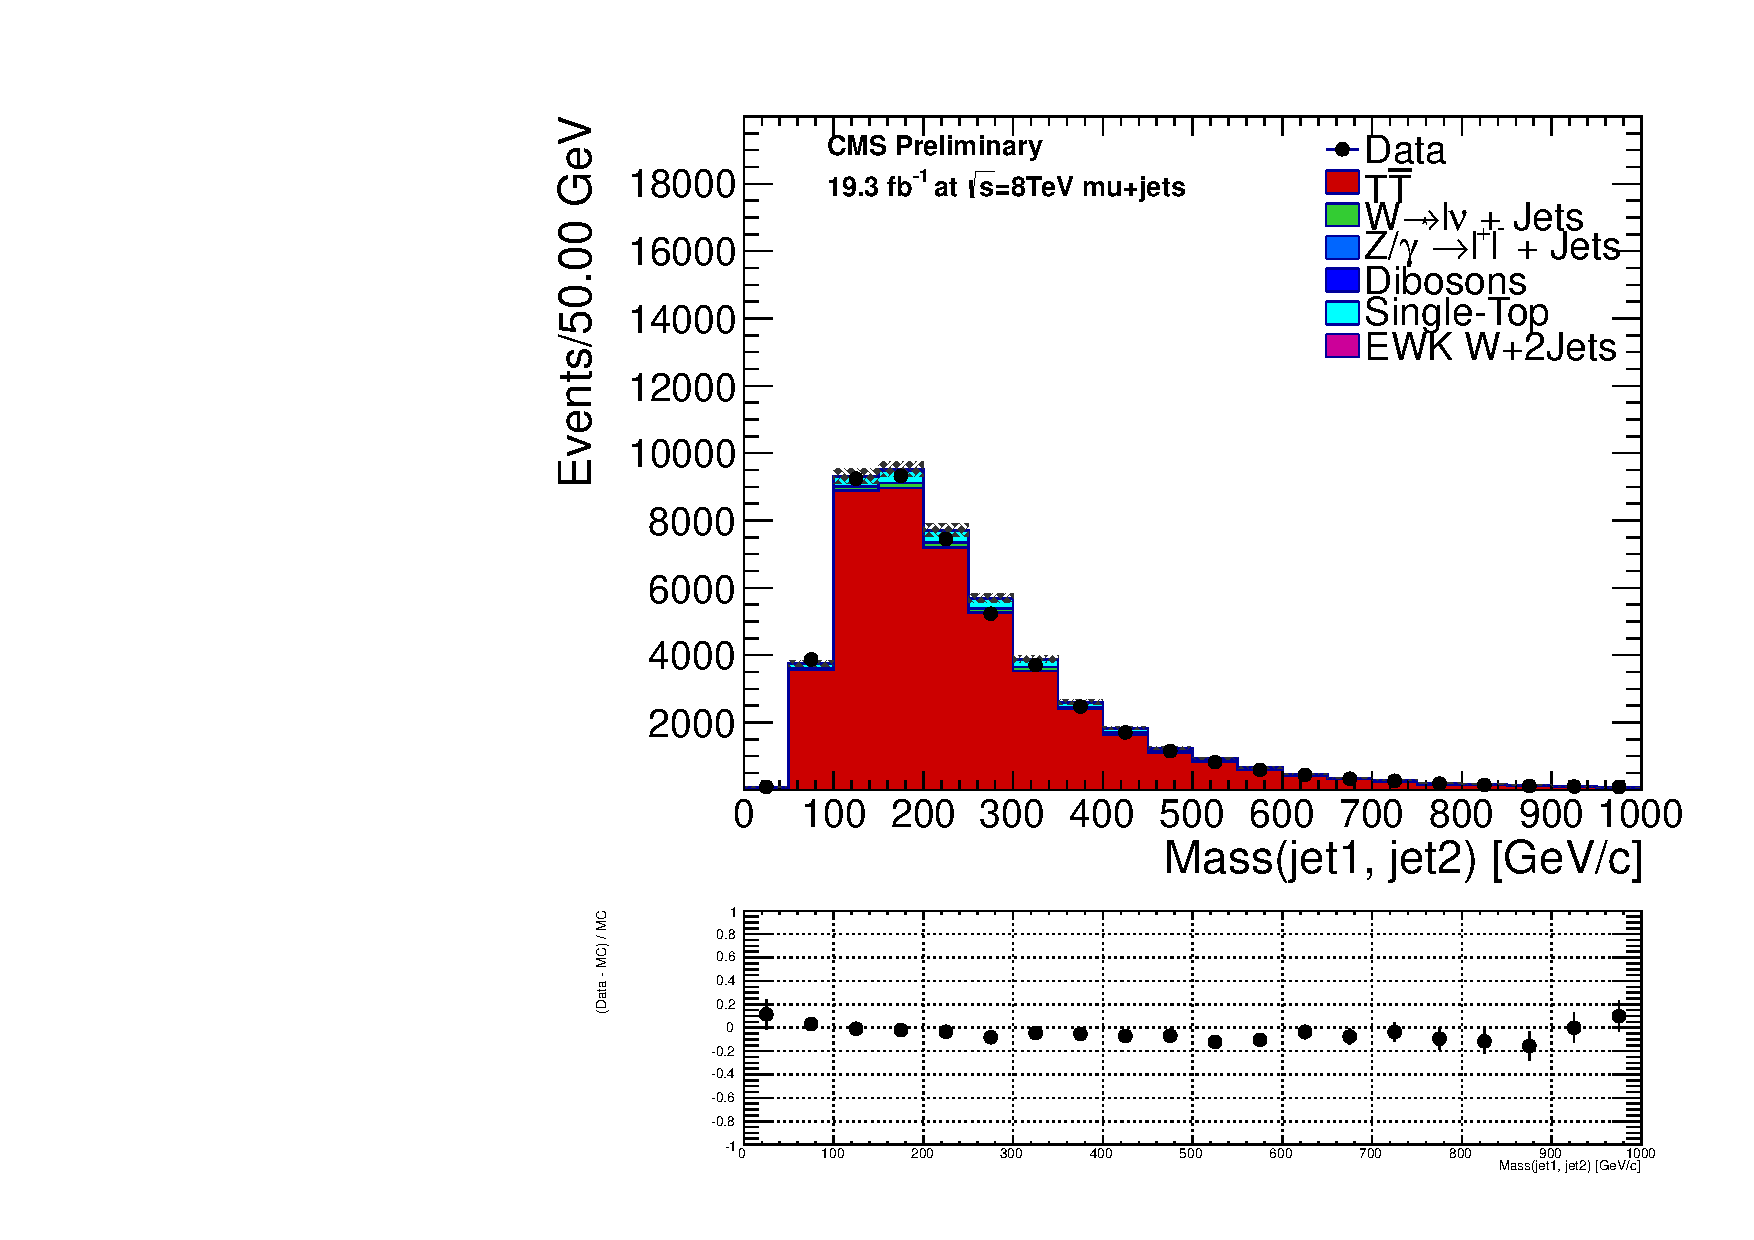
\includegraphics[width=0.49\textwidth]{figs/topwjes/mu_EWK_W_2jets_ttbar_firstsecondmjj_TTbarControlPlots_EWKW2jets.pdf}
    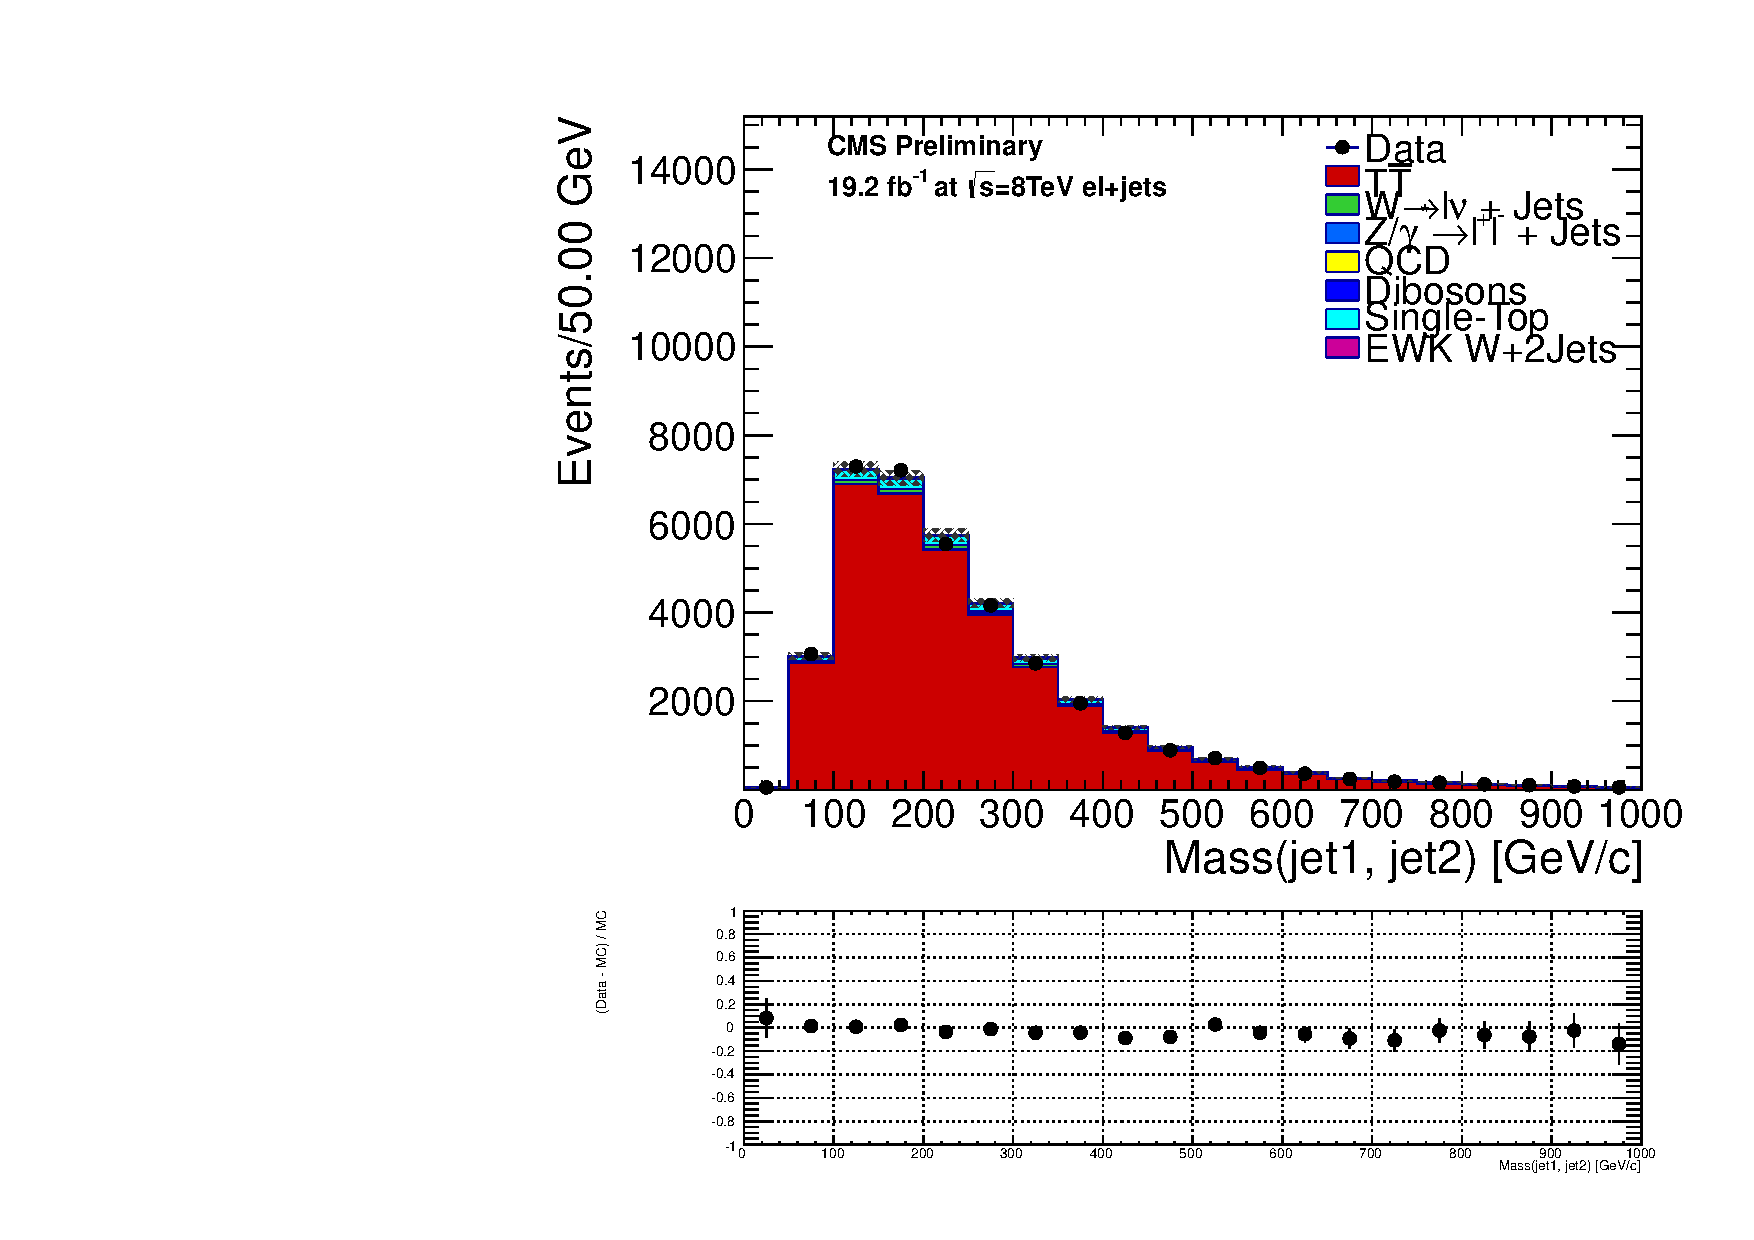
\includegraphics[width=0.49\textwidth]{figs/topwjes/el_EWK_W_2jets_ttbar_firstsecondmjj_TTbarControlPlots_met_30_WmT_30_EWKW2jets.pdf}
    \caption{The invariant mass distribution of the leading jet and second leading jet in the semileptonic top control sample: muons (left) and electrons (right).}
    \label{fig:topw:mu_MC}}
\end{figure}
%%%%%%%%%%%%%%
\begin{figure}[htb] 
  {\centering
    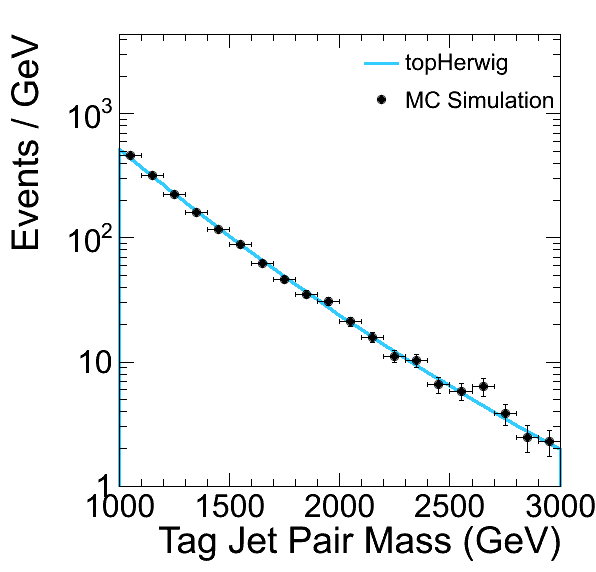
\includegraphics[width=0.49\textwidth]{figs/wpj/EWKW2jetstagjetmjj_topHerwig_defaultfit_muon_Model_12_Validate.png}
    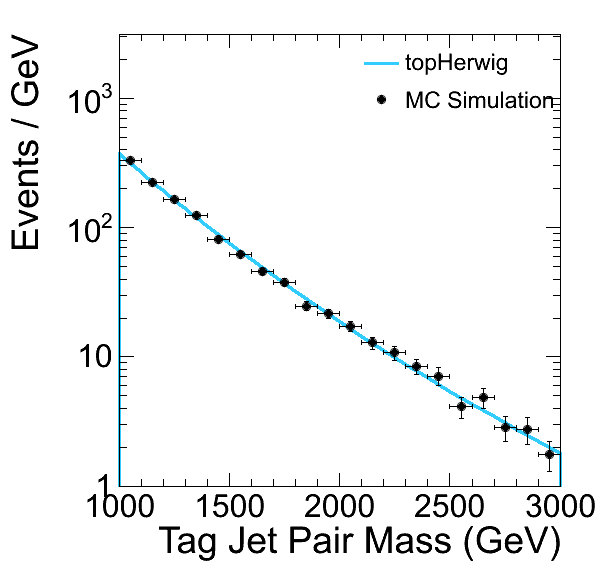
\includegraphics[width=0.49\textwidth]{figs/wpj/EWKW2jetstagjetmjj_topHerwig_defaultfit_electron_Model_12_Validate.png}
    \caption{Top aMC@NLO tag jet pair mass $m_{jj}$ shape: projection of a fit to the Top aMC@NLO MC for muons (left) and electrons (right).}
    \label{fig:mu_MC_topaMCNLO}}
\end{figure}
%%%%%%%%%%%%%%
\begin{figure}
\begin{center}
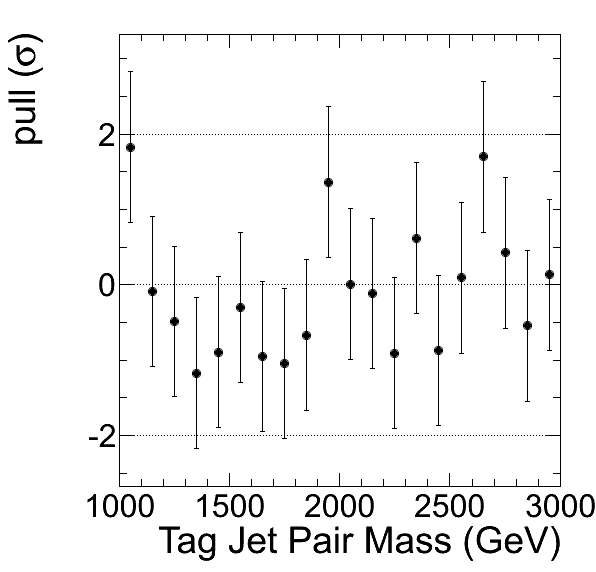
\includegraphics[width=0.45\textwidth]{figs/wpj/EWKW2jetstagjetmjj_topHerwig_defaultfit_muon_Model_12_Validate_pull.png}
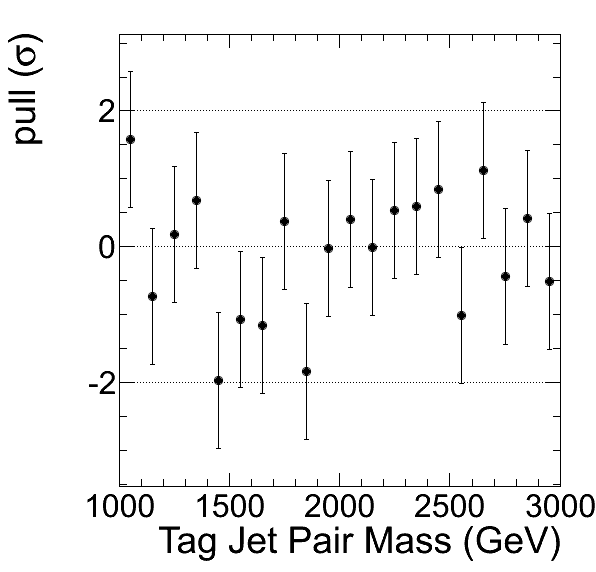
\includegraphics[width=0.45\textwidth]{figs/wpj/EWKW2jetstagjetmjj_topHerwig_defaultfit_electron_Model_12_Validate_pull.png}
\end{center}
\caption{Top aMC@NLO tag jet pair mass $m_{jj}$ shape: Pull distribution of a fit to the Top aMC@NLO MC for muons (left) and electrons (right).}
\label{fig:mu_MC_topaMCNLO_pull}
\end{figure}
%%%%%%%%%%%%%%
\begin{figure}[htb] 
  {\centering
    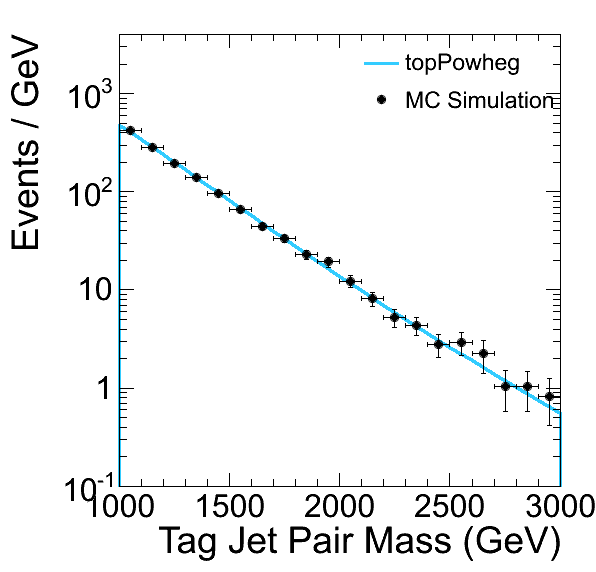
\includegraphics[width=0.49\textwidth]{figs/wpj/EWKW2jetstagjetmjj_topPowheg_defaultfit_muon_Model_12_Validate.png}
    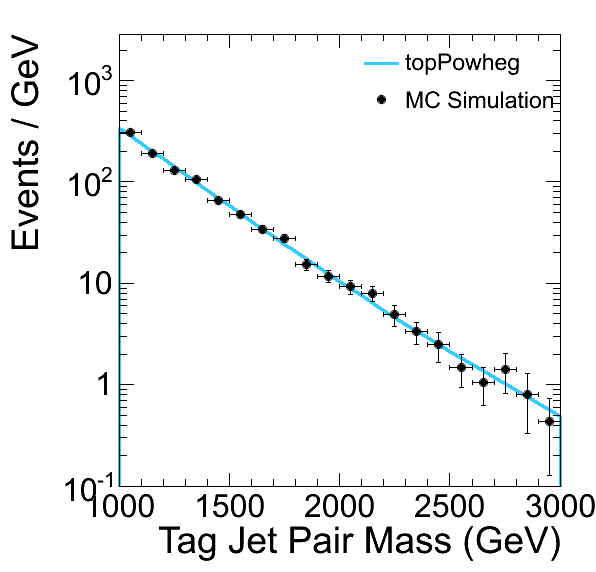
\includegraphics[width=0.49\textwidth]{figs/wpj/EWKW2jetstagjetmjj_topPowheg_defaultfit_electron_Model_12_Validate.png}
    \caption{Top Powheg tag jet pair mass $m_{jj}$ shape: projection of a fit to the Top Powheg MC for muons (left) and electrons (right).}
    \label{fig:mu_MC_toppowheg}}
\end{figure}
%%%%%%%%%%%%%%
\begin{figure}[htb] 
  {\centering
    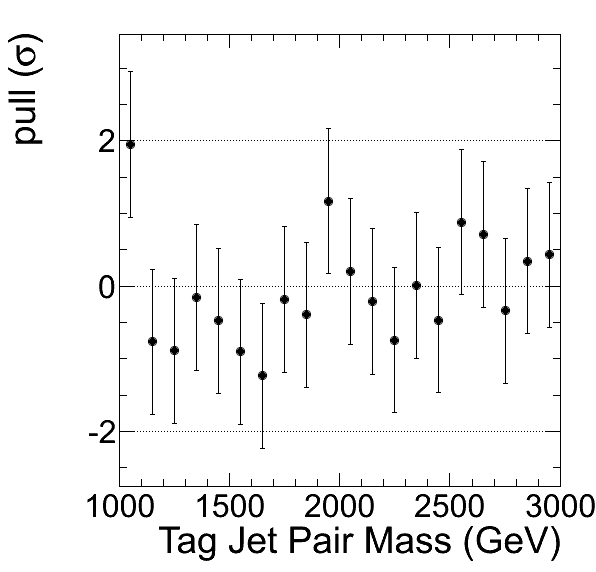
\includegraphics[width=0.49\textwidth]{figs/wpj/EWKW2jetstagjetmjj_topPowheg_defaultfit_muon_Model_12_Validate_pull.png}
    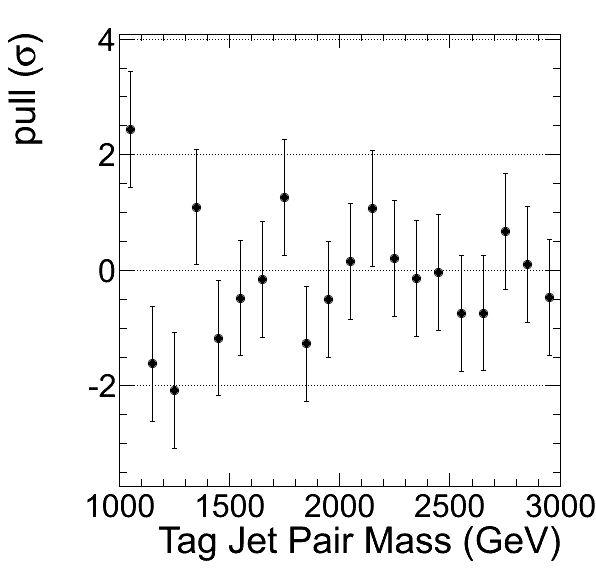
\includegraphics[width=0.49\textwidth]{figs/wpj/EWKW2jetstagjetmjj_topPowheg_defaultfit_electron_Model_12_Validate_pull.png}
    \caption{Top Powheg tag jet pair mass $m_{jj}$ shape: Pull distribution  of a fit to the Top Powheg MC for muons (left) and electrons (right).}
    \label{fig:mu_MC_toppowheg_pull}}
\end{figure}
%%%%%%%%%%%%%%%%%%%%%%%%%
%--------------------------------------------------
\subsection{Lepton selection and trigger efficiency}
\label{sec:LeptonSelectionAndTriggerEfficiency}
%%The lepton trigger and selection is common among several CMS analyses and 
%%we benefit from common studies based on tag-and-probe techniques. 
%%
Systematic uncertainties in the trigger efficiencies in
Section~\ref{sec:Eff} are of the order of 1\%. Systematic
uncertainties in the lepton reconstruction and identification
efficiency scale factors are of the order of 2\%. 
%These uncertainties
%are accounted for in the final systematics that are input to the
%cross-section uncertainty calculation.
%--------------------------------------------------
\subsection{MET uncertainty}
MET directly affects our signal acceptance. 
The uncertainty prescription is discussed in Ref.~\cite{met}.
%https://twiki.cern.ch/twiki/bin/viewauth/CMS/MissingETUncertaintyPrescription
In addition, the MET distribution in the data is $\simeq$3\% wider 
than the MC, and placing a hard MET$>30.0$ cut creates an uncertainty. 
We estimate it by smearing the MET for each event by a Gaussian with 
a $\sigma =0.03*$MET and observing how many events pass the cut. 
Specifically, (Events Passing After Smearing)/(Events Passing Before Smearing) 
=0.998 for both muons and electrons.
%%%%%%%%%%%%%%%%%%%%%%%%%%%%
\subsection{Cross-section of minor backgrounds}
The uncertainties in the cross sections of other minor backgrounds 
like Diboson and Z+jets processes are negligible in this analysis.
%already propagated by letting their new normalization (i.e., yield$\pm1\sigma$) in the fit.

%%%%%%%%%%%%%%%%%%%%%%%%%%%%%
%\subsection{Theory uncertainty in acceptance}
%The theory uncertainty on the signal acceptance due to variations in the parton distribution functions and the
%value of $\alpha_{s}$ is obtained by following the {\sc pdf4lhc} prescription ~\cite{Botje:2011sn}.
%Using \textsc{CT10}~\cite{ct10}, \textsc{MSTW08}~\cite{Martin:2009iq}, and \textsc{NNPDF}~\cite{nnpdf} sets, the uncertainties are estimated to be XX\% 
%%for $q\bar{q} \to WW$ and and 0.8\% for $gg \to WW$ by the leptonic $WW$ group (SMP-12-024).
%
%Likewise, the impact of higher-order corrections is estimated by varying the QCD renormalisation
%($\mu_R$) and factorization ($\mu_F$) scales up and down by a factor of two using the \textsc{mcfm} program~\cite{MCFMarticle} and found to be 1.5\%. 
%The overall theory uncertainty is below 3\%, consistent with our studies at 7~TeV (AN-12-224).


%For the 7TeV analysis we compute theory uncertainty in acceptance for muon ``no b-tag'' selection 
%using MCFM: $\pt^{\text{jet}}>35$~GeV, $|\eta^{\text{jet}}|<2.4$, 
%$\pt^{\text{lepton}}>325$~GeV, $|\eta^{\text{lepton}}|<2.1$, 
%$\met > 30$~GeV, W $m_T > 30$~GeV, $\Delta{R}$ (lepton, jet) $>0.3$, 
%no additional lepton. 
%We use CTEQ6.6m as the default PDF and the quantity $\mu_0 = \sqrt{M_W^2 + p_{T, W}^2}$ as  
%the default factorization/renormalization scale.
%For systematic studies 
%we vary the choices of PDF and the factorization/renormalization 
%scale. The details are shown in Table~\ref{tab:theorysyst}. 
%The overall theory 
%uncertainty is below 3\%.
% %%%%%%%%%%%%%%%%%%%%%%%%%%%
% \begin{table}[h!]
%   \begin{center}
%   \begin{tabular}{l|c}
%  \hline
%  \hline
%  Source of uncertainty & Relative variation in acceptance value \\
%  \hline                                  
%  PDF: CT10                             & $1.4\%$ \\
%  PDF: CTEQ61M                          & $-0.7\%$ \\
%  PDF: MSTW8NL                          & $0.4\%$ \\
%  PDF: MSTW8NN                          & $0.1\%$ \\
%  PDF: MSTW8LO                          & $-1.3\%$ \\
%  Scale: $2~\mu_0$                      & $-0.01\%$ \\
%  Scale: $0.5~\mu_0$                    & $0.8\%$ \\
%  Scale: $\sqrt{M_W^2 + p_{T, jet1}^2}$ & $-0.3\%$ \\
%  Scale: $H_T$                          & $0.1\%$ \\
%  \hline
%  \hline
%   \end{tabular}
%   \end{center}
%   \caption{Theory uncertainty in acceptance. The central value for 
%   acceptance $\times$ branching fraction is $(1.279 \pm 0.019) \times 10^{-2}$.} 
%   \label{tab:theorysyst}
% \end{table}
% %%%%%%%%%%%%%%%%%%%%%%%%%
%%%%%%%%%%%%%%%%%%%%%%%%%%%%
%\subsection{Uncertainty in jet veto efficiency}
%Since we use events with exactly two jets, we reject signal events 
%which have extra jet(s) from ISR or FSR. Our acceptance computation 
%takes this inefficiency into account. However, there is a 
%systematic uncertainty associated with the modeling of 
%ISR/FSR in our simulation. The effect has been studied by the WW group and is expected to be less than 5\% (SMP-12-024).

%For the 7TeV analysis, to estimate this systematics we 
%compare the efficiency of our jet veto at generator-level 
%(i.e., using ``GenJets'') in the Pythia WW, Pythia WZ, and 
%privately produced MadGraph WW samples. All three simulations 
%use LO matrix element calculation, parton showering from 
%Pythia, and identical choices of factorization/renormalization
%scales and PDFs. However, the soft gluon radiation probability 
%is different in each sample.  
%Table~\ref{tab:jetvetoeff} lists the jet-veto efficiency 
%in each of the three samples. We take the maximum 
%difference in efficiency as a systematic uncertainty.
%This systematic is within 2\%.
%%%%%%%%%%%%%%%%%%%%%%%%%%%
% \begin{table}[h!]
%   \begin{center}
%   \begin{tabular}{l|c}
%  \hline
%  \hline
%  Sample & jet-veto efficiency \\
%  \hline                                  
%  WW Pythia                             & $88.72\%$ \\
%  WZ Pythia                             & $87.48\%$ \\
%  WW MadGraph                           & $89.57\%$ \\
%  \hline
%  \hline
%   \end{tabular}
%   \end{center}
%   \caption{Jet-veto efficiency in various diboson simulations.} 
%   \label{tab:jetvetoeff}
% \end{table}
%%%%%%%%%%%%%%%%%%%%%%%%%%
%%%%%%%%%%%%%%%%%%%%%%%%%%%%
\subsection{Interference effect between EWK W+2jets and QCD W+2jets background}
\label{sec:interefence}
EWK W+2jets and QCD W+2jets interference effect may change the signal MC shape in the fit. In order to account this effect, three samples have been generated:
\begin{itemize}
\item  EWK W+2jets sample: QCD=0 in MadGraph
\item  QCD W+2jets sample: QCD=2 QED=2 in MadGraph
\item  EWK W+2jets + QCD W+2jets + interference effect sample: QCD=2 QED=4 in MadGraph
\end{itemize}
Then our default EWK W+2jets shape is replaced by the shape including both EWK W+2jets and interference effect in the fit. The interference effect is shown in Figs~\ref{fig:interference}. The two parameter power function to model the EWK W+2jets plus interference effect is also shown in Figs~\ref{fig:interference}.

\begin{figure}[htb] 
  {\centering
    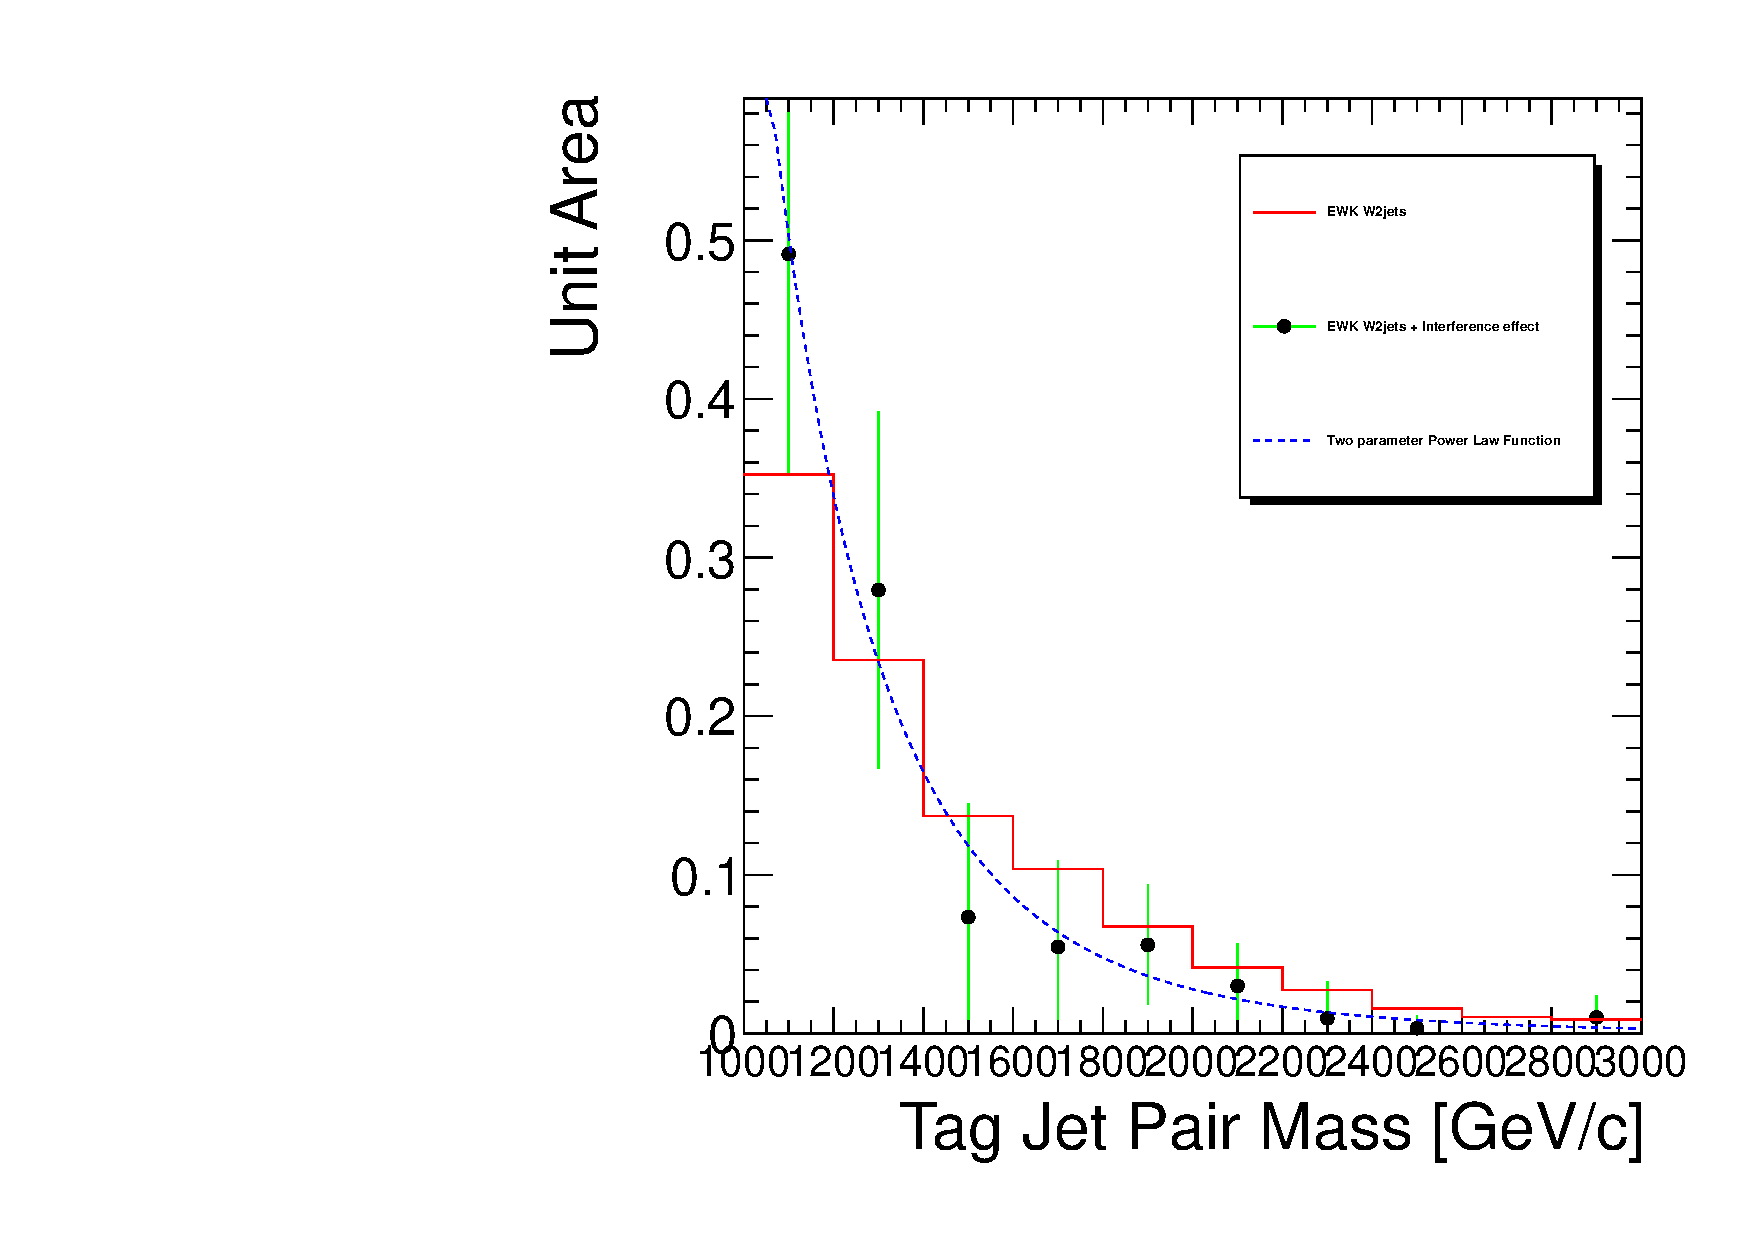
\includegraphics[width=0.49\textwidth]{figs/systematic/mu_tagjet_massinterference10003000_EWKOverinterferenceUnitArea.pdf}
    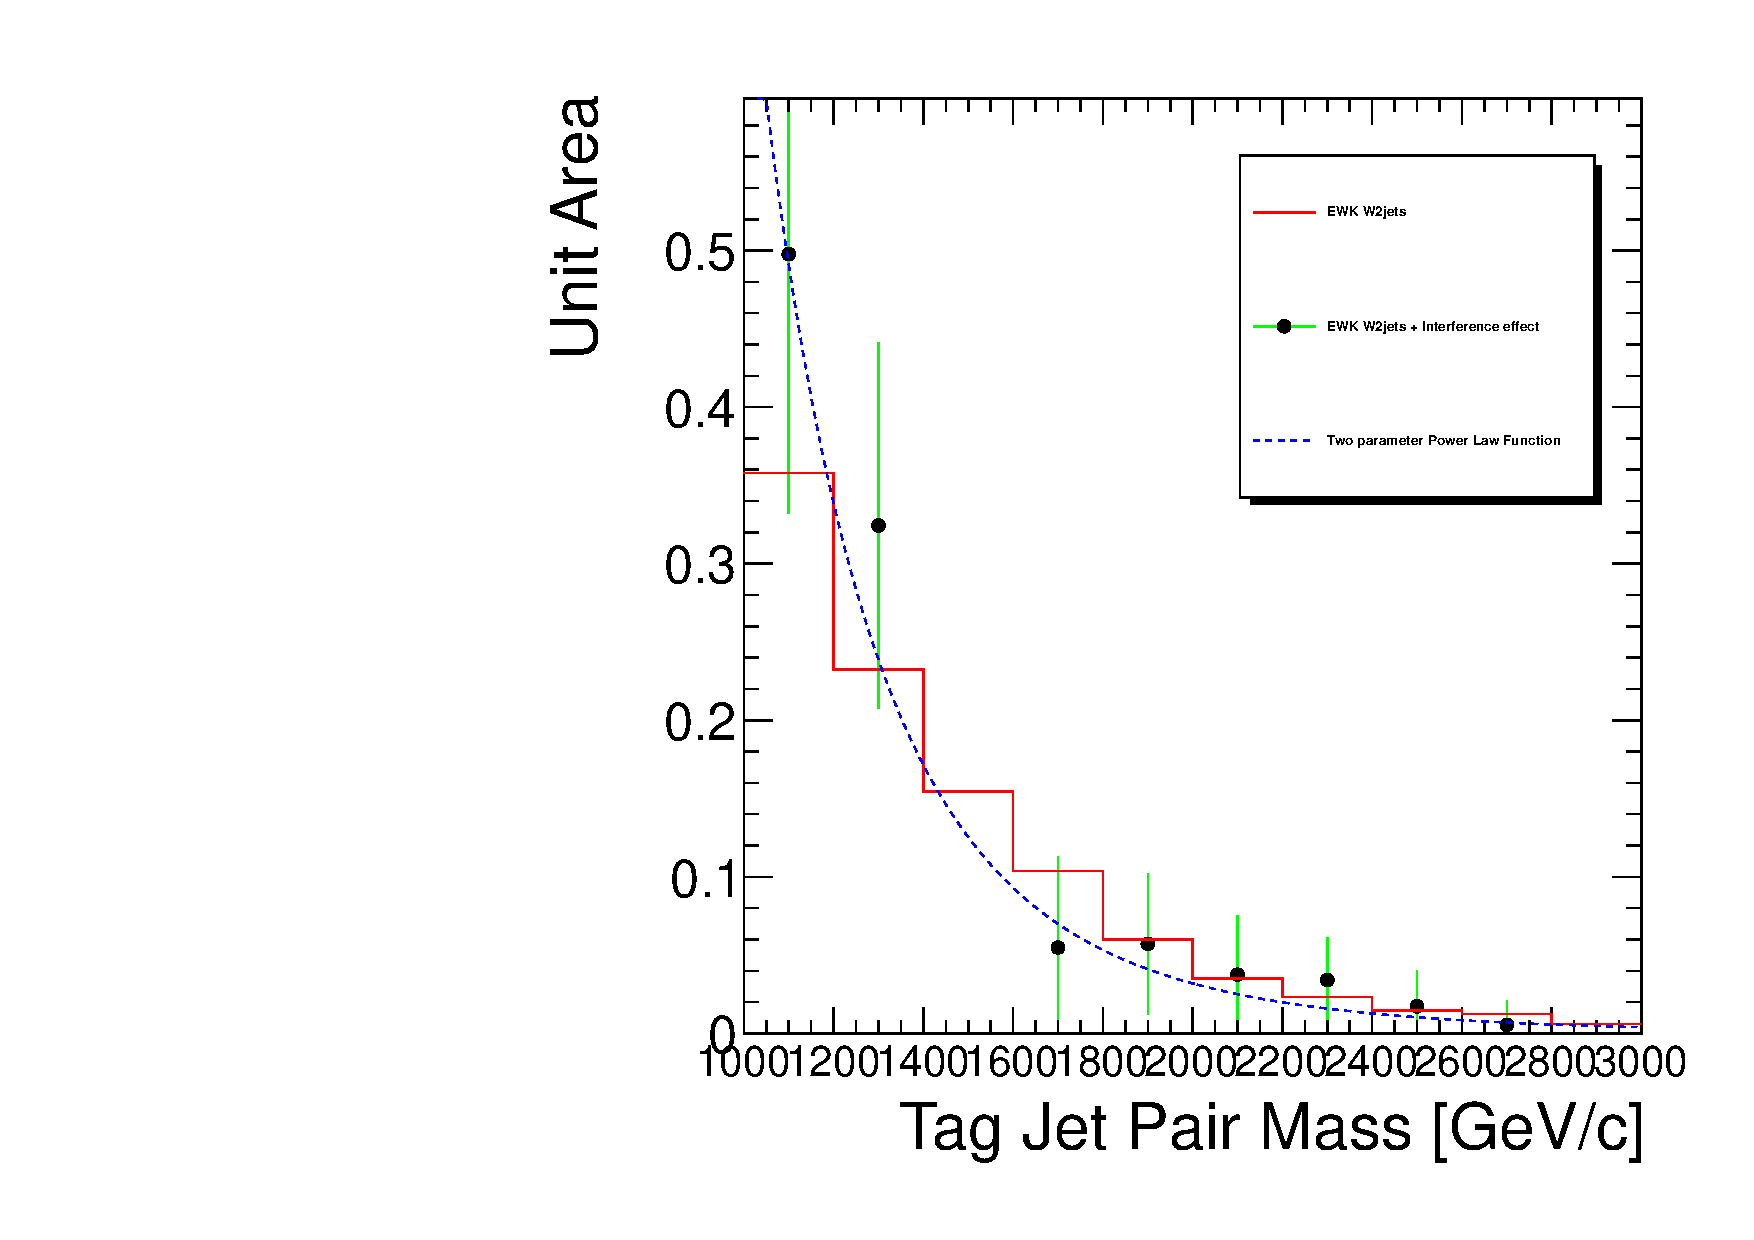
\includegraphics[width=0.49\textwidth]{figs/systematic/el_tagjet_massinterference10003000_EWKOverinterferenceUnitArea.pdf}
    \caption{Shape comparison between EWK W+2jets and EWK W+2jets plus interference effect for muons (left) and electrons (right). The two parameter power law function to model the EWK W+2jets plus interference effect for muons (left) and electrons (right)}
    \label{fig:interference}}
\end{figure}

%%%%%%%%%%%%%%%%%%%%%%%%%%%
\subsection{QCD fraction prediction in the electron channel}
QCD fraction estimation is described in Section~\ref{sec:qcd} with 50\% conservative uncertainty assigned. Then we vary the QCD fraction estimation by $\pm50\%$ in the electron channel fit.

%%%%%%%%%%%%%%%%%%%%%%%%%%%%%%
\subsection{Luminosity uncertainty}
\label{sec:LumiUncertainty}
The latest recommendation for the uncertainty on LHC luminosity is 4.4$\%$~\cite{lumiPAS}.
We propagate this uncertainty to the expected yield of the signal and from there to the
calculated cross-section.
%%%%%%%%%%%%%%%%%%%%%%%%%%%%
%%%%%%%%%%%%%%%%%%%%%%%%%
 \begin{table}[h!]
   \begin{center}
   \begin{tabular}{l|c|c}
  \hline
  \hline
  Source of uncertainty & Muons & Electrons \\
  \hline                                  
  Luminosity                             & 0.044 & 0.041 \\
  \hline 
  Jet energy scale & 0.043 & 0.051\\
  Jet energy resolution & 0.108 & 0.108 \\
%  Jet energy scale & 0.095 & 0.097\\
%  Jet energy resolution & 0.252 & 0.271 \\
  W+jets shape and normalization & 0.062 & 0.066\\
  TTbar shape and normalization & 0.052 & 0.046\\
  Interference effect & 0.064 & 0.070\\
  %Theory acceptances (PDF)               &  & \\
  %ISR/FSR acceptances                    &  & \\
  QCD fraction prediction(electron channel) & ---- & 0.042\\
  Lepton trigger eff.                    & 0.010 & 0.009 \\
  Lepton selection eff.                  & 0.020 & 0.018 \\
  Pile-up                                & $<1\%$ & $<1\%$ \\
  \hline 
  total (without Luminosity)             & 0.157 & 0.167\\
  \hline
  \hline
   \end{tabular}
   \end{center}
   \caption{Sources of systematics considered in the analysis, with the corresponding magnitude on the signal strength.} 
   \label{tab:signalSyst}
 \end{table}
%%%%%%%%%%%%%%%%%%%%%%%%%
